\documentclass{article}
\usepackage{figsize}


\title{The FigSize Package}
\author{Anthony A. Tanbakuchi \\{\small atanbakuchi@hotmail.com} \\ v0.1 last revised 2002/3/18}
\date{}

\parskip=12pt
\parindent=0pt
\begin{document}
\maketitle
\begin{abstract}
The FigSize package enables automatic sizing of graphics,
especially when including graphics with the graphicx package.  The
user only has to specify the number of graphics that should fit to
a page or fraction there of and the package will dynamically
calculate the correct graphics sizes relative to the page size.
Thus, graphics can be auto-sized to fill a whole page or fraction
and manual changes of graphic sizes are never needed when changing
document layouts!  Finally, the package's dynamic lengths can be
used to allow other document element sizes to be dynamic.
\end{abstract}

\section{Usage}

Perhaps the best way to see how this package works is to skip to
the examples section.  However, below is a more general
explanation of the package and its use.

Loading the package:

    \verb"\loadpackage{figsize}"\\

Next, to allow the FigSize package to dynamically define widths
and heights for the graphic simply specify the desired layout
using,


    \verb"\SetFigLayout[<extra space for long captions>]{<rows>}{<columns>}".

Where you specify the number of rows and columns of graphics that
should fit to a page.  Optionally, if you have a long caption you
can tell the package how many extra lines of text that should be
allowed for on the page as well.

Then, just include the graphic using the command from the graphicx
package (which is just the advanced version of the graphics
package),

\verb"\includegraphics{filename}"\footnote{For a detailed
explanation on how to use the graphics package and the
$\backslash$includegraphics command see the guide to using
graphics with \LaTeX. Found online at
http://www.ctan.org/tex-archive/help/Catalogue/entries/grfguide.html?}

Thus, if one issues the command \verb"\SetFigLayout{2}{1}" the
algorithm knows that any graphics inserted after this point with
the command \verb"\includegraphics{...}" should be sized so that
two high by one wide will fit on a page.

When \verb"\SetFigLayout{}{}" is issued the package redefines two
new page relative lengths \verb"\figwidth" and \verb"\figheight".
Then, \verb"\includegraphics{...}" is redefined to by default have
optional parameters set to \\
    \verb"[width=\figwidth, totalheight=\figheight, keepaspectratio]".

By default, this package makes the assumption that figures should
be resized while keeping their aspect ratio.  This may not be the
desired effect, to remove this effect insert figures using,\\
    \verb"\includegraphics[width=\figwidth, totalheight=\figheight]{...}"\\
\noindent Further, one can utilize all the optional facilities
provided by the \verb"\includegraphics{...}" command, simply use
the format,\\
    \verb"\includegraphics[width=\figwidth, totalheight=\figheight, <more options>]{...}"

Moreover, one can use the new dynamic widths \verb"\figwidth" and
\verb"\figheight" for other types of environments like tables,
pictures, and so on.

\section{Package Requirements}
When the FigSize package is loaded  it loads the
\textbf{subfigure}, \textbf{graphicx}, \textbf{ifthen}, and
\textbf{calc} packages.  These packages must already exist on the
\LaTeX system for the FigSize package to work properly.

\section{Examples}

The best way to see how this package works is through examples.
The next few examples illustrate common uses for the FigSize
package.

The following code sets the size of the graphics so that 4 rows by
3 columns of them fit to a page. The result is shown in Figure
\ref{fig:1} and \ref{fig:1b}.

\begin{verbatim}
\begin{figure}
\SetFigLayout{3}{3}
    \subfigure[A subfigure.]{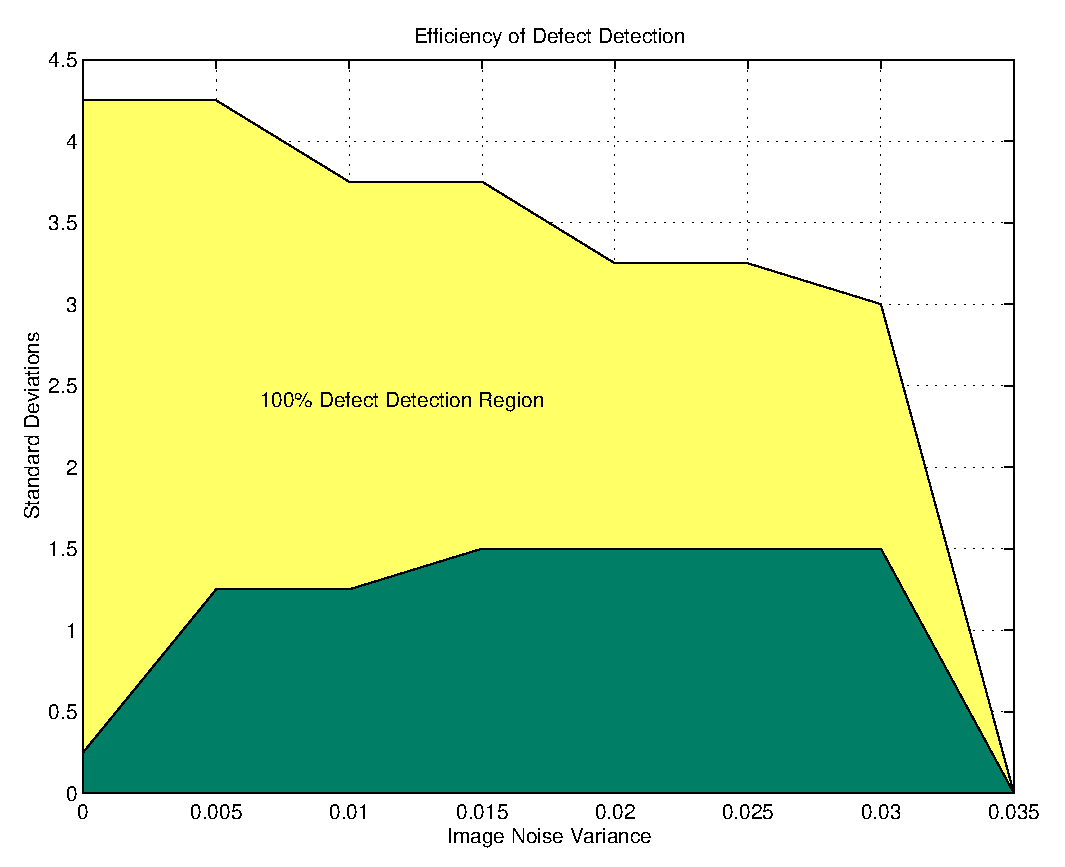
\includegraphics{epsfig}}
    \hfill
    \subfigure[A subfigure.]{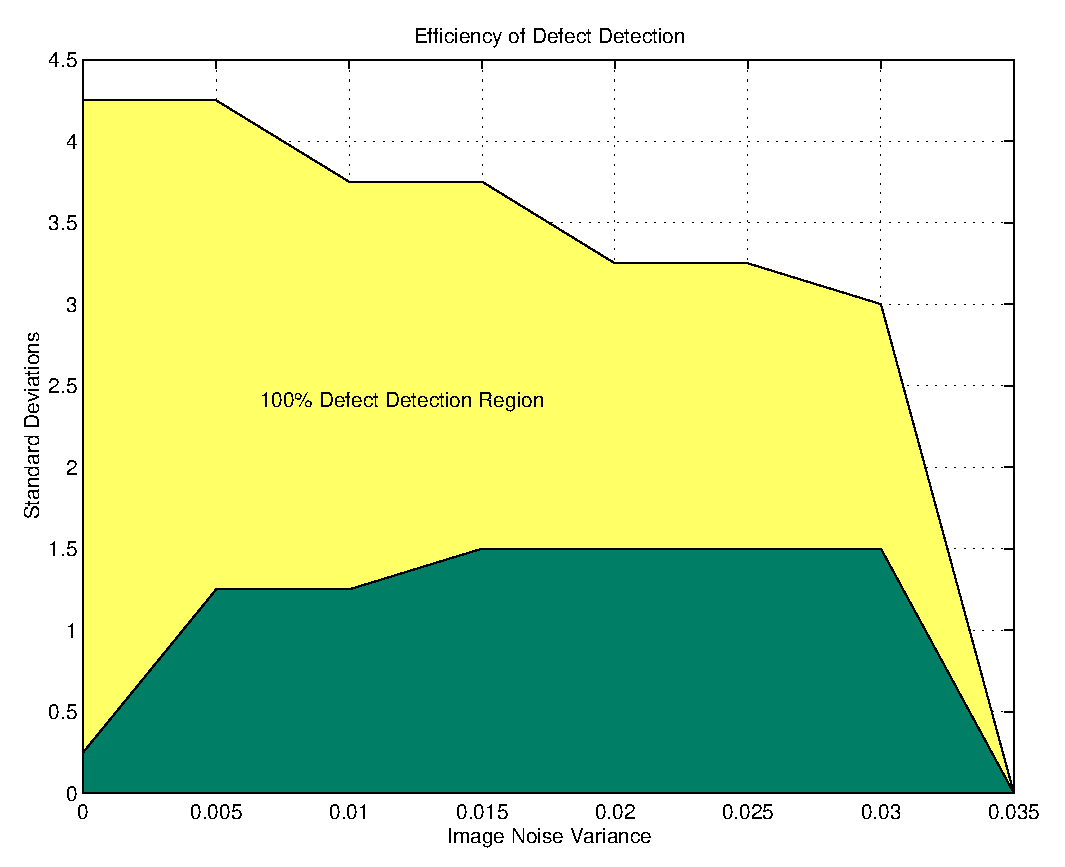
\includegraphics{epsfig}}
    \hfill
    \subfigure[A subfigure.]{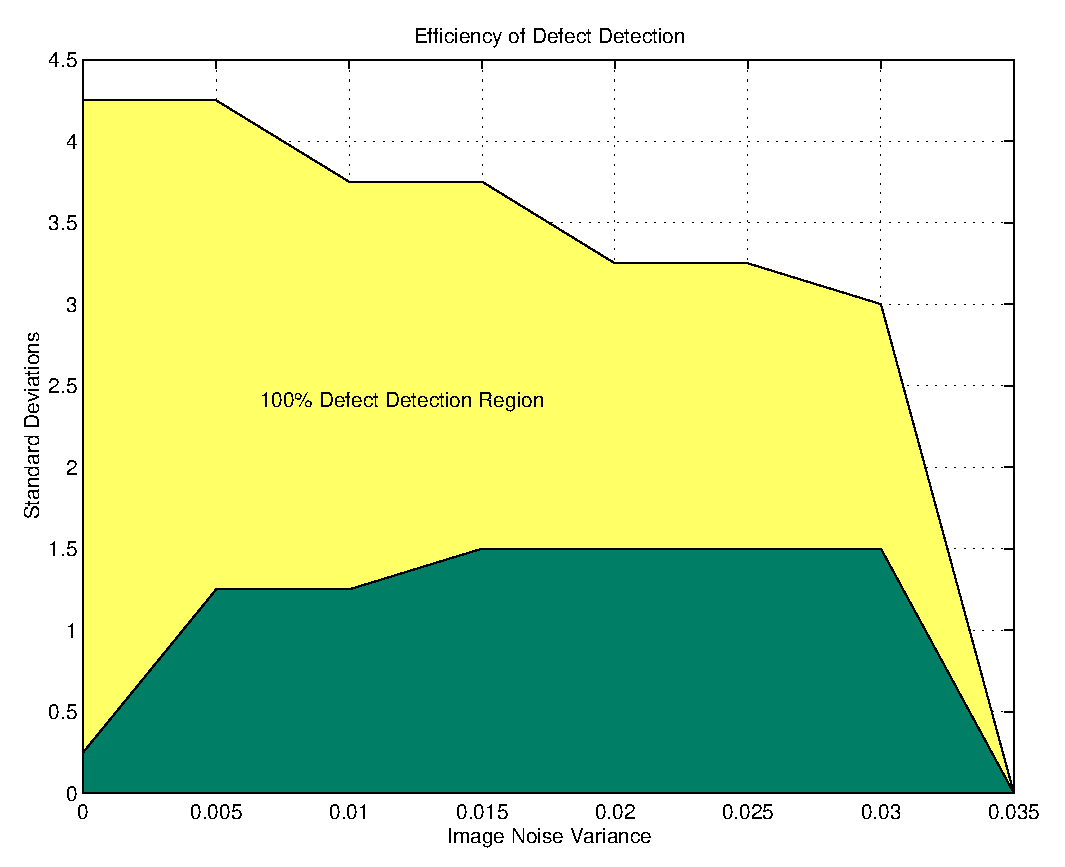
\includegraphics{epsfig}} \\
    \subfigure[A subfigure.]{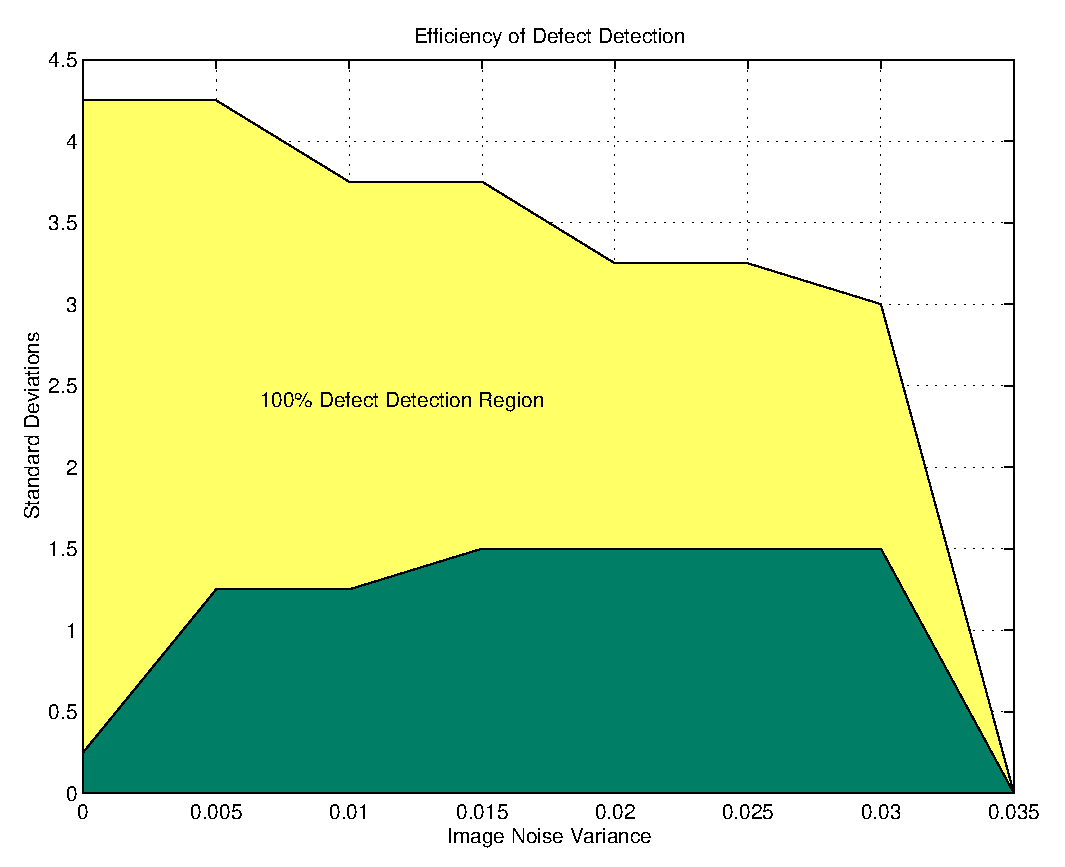
\includegraphics{epsfig}}
    \hfill
    \subfigure[A subfigure.]{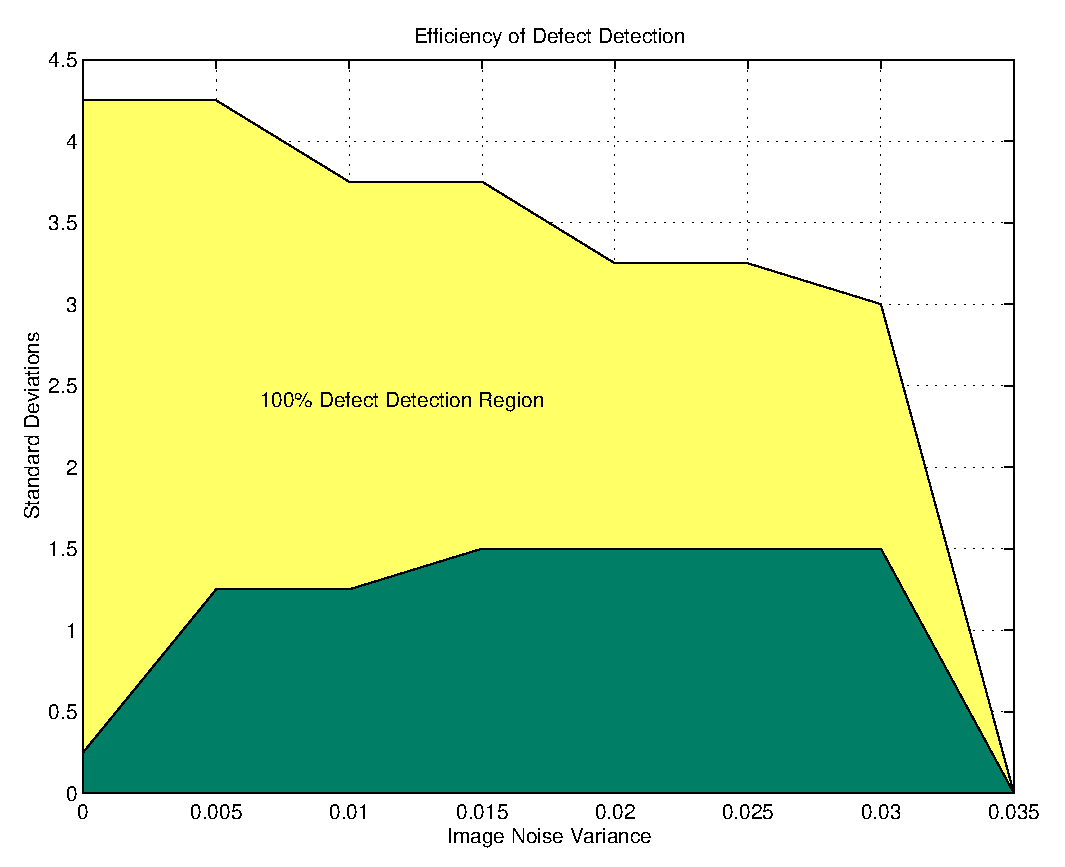
\includegraphics{epsfig}}
    \hfill
    \subfigure[A subfigure.]{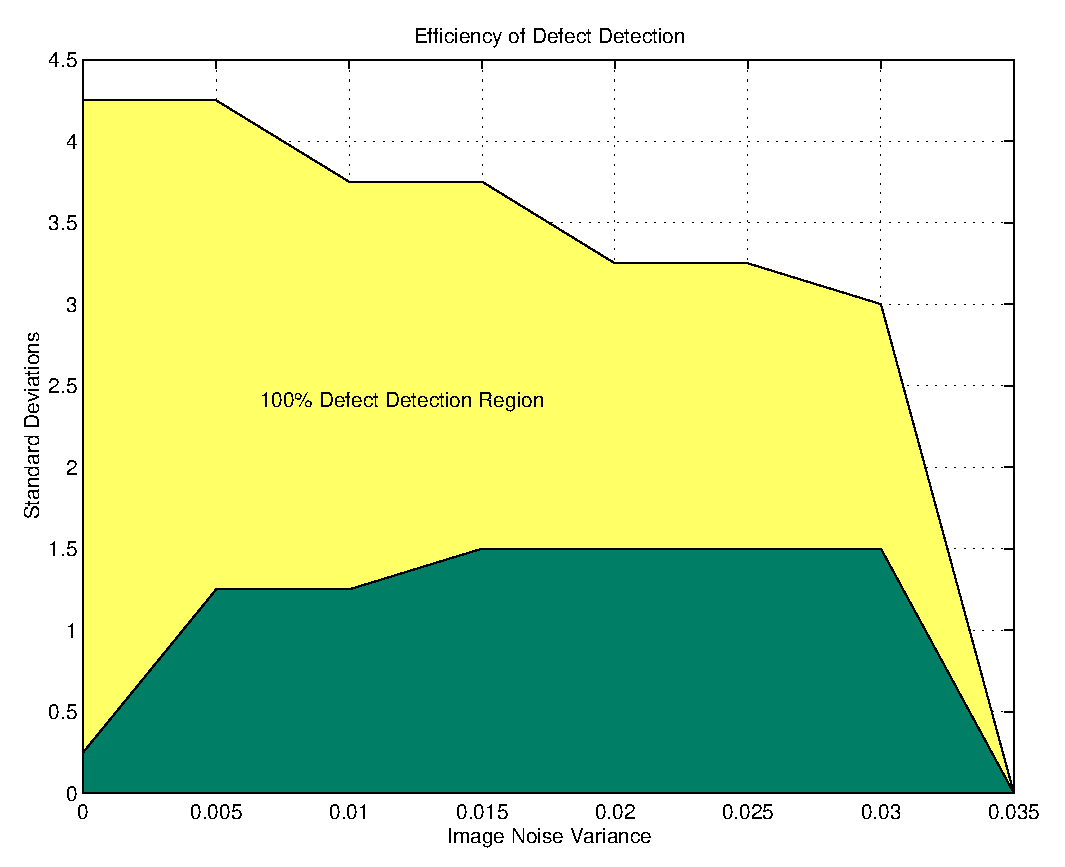
\includegraphics{epsfig}} \\
    \subfigure[A subfigure.]{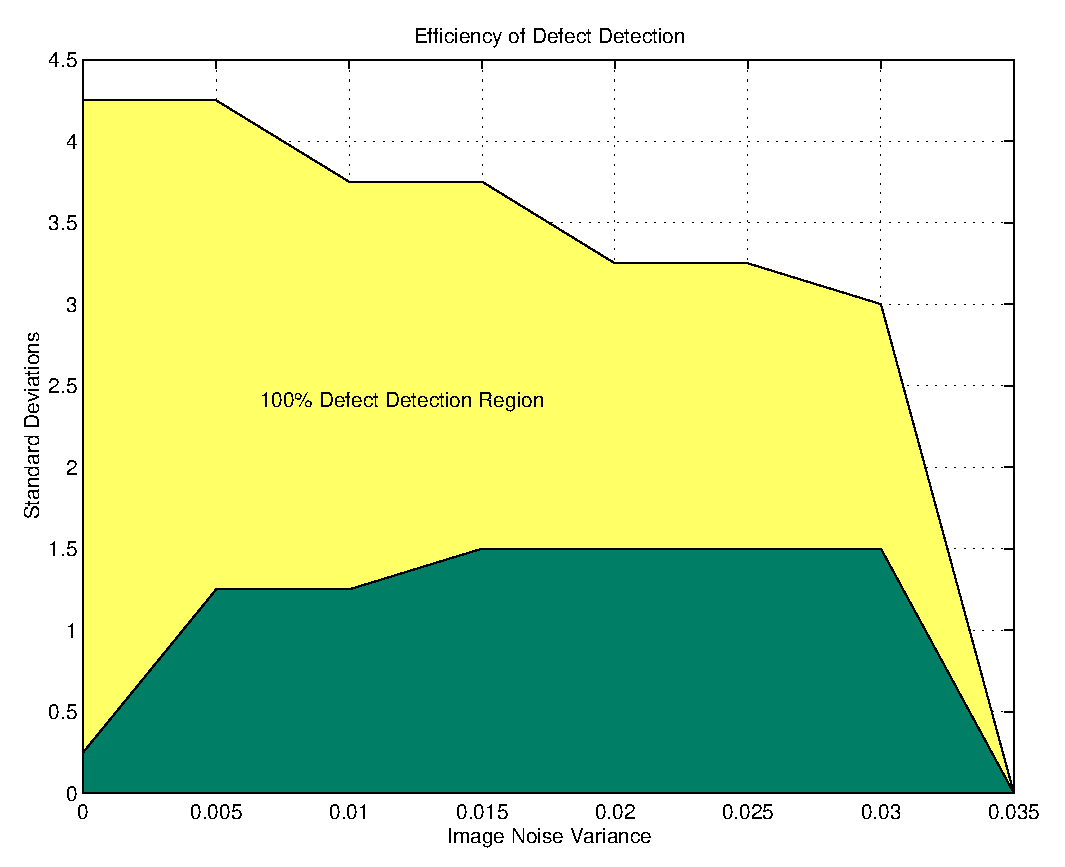
\includegraphics{epsfig}}
    \hfill
    \subfigure[A subfigure.]{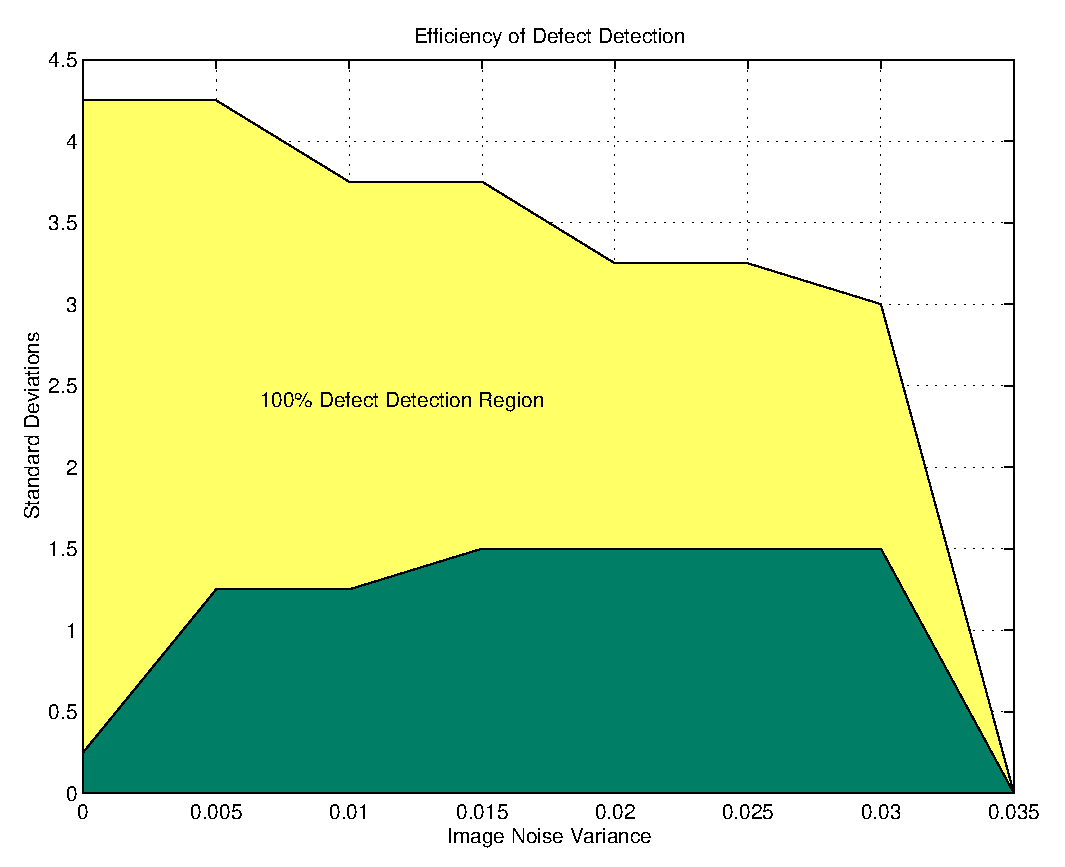
\includegraphics{epsfig}}
    \hfill
    \subfigure[A subfigure.]{
    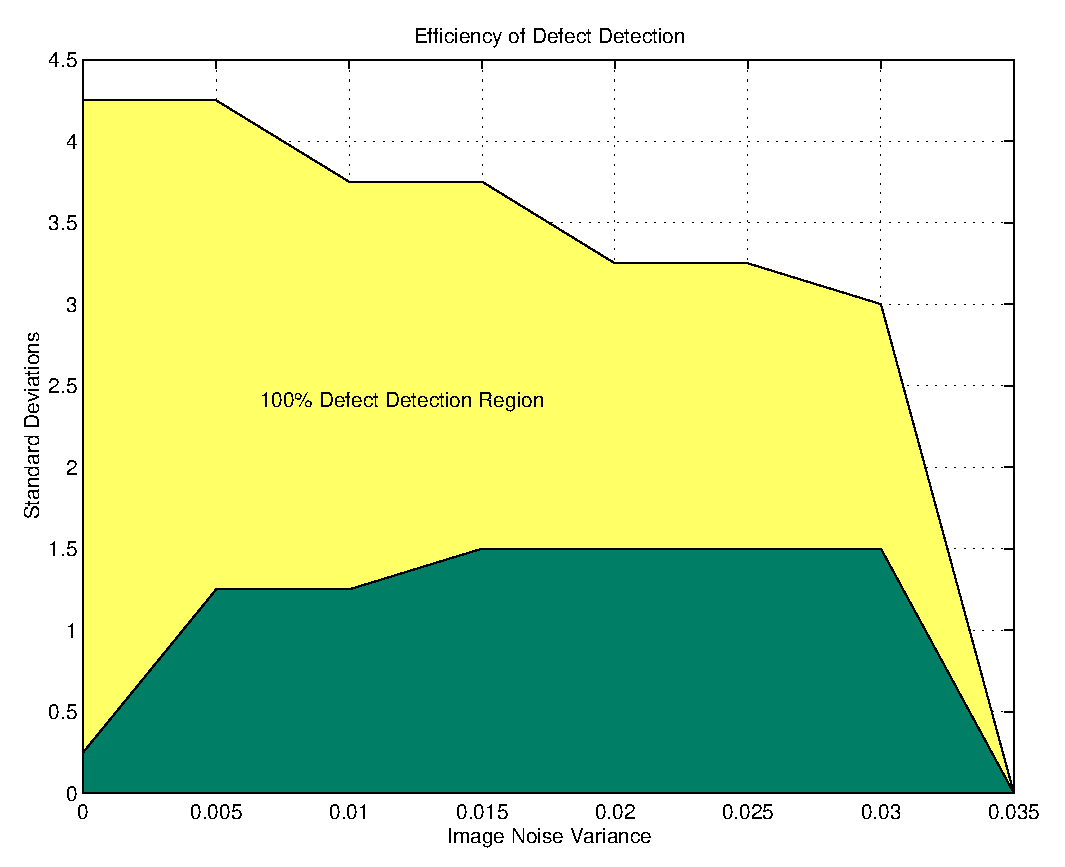
\includegraphics[angle=45, width=\figwidth,
    totalheight=\figheight, keepaspectratio]{epsfig}}

    \caption{This is where your caption text goes. No
    optional parameters.}\label{fig:1}
\end{figure}

\begin{figure}
\SetFigLayout{3}{3}
    \subfigure[A subfigure.]{
    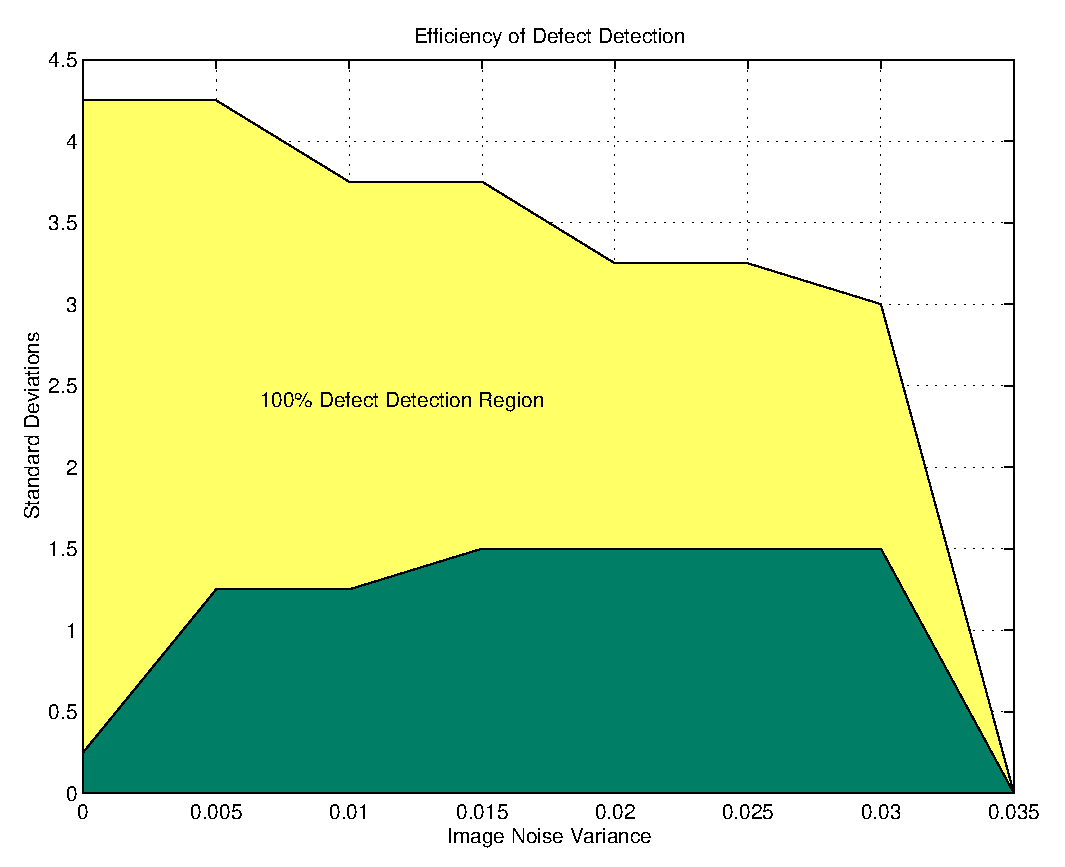
\includegraphics[width=\figwidth, totalheight=\figheight]{epsfig}}
    \hfill
    \subfigure[A subfigure.]{
    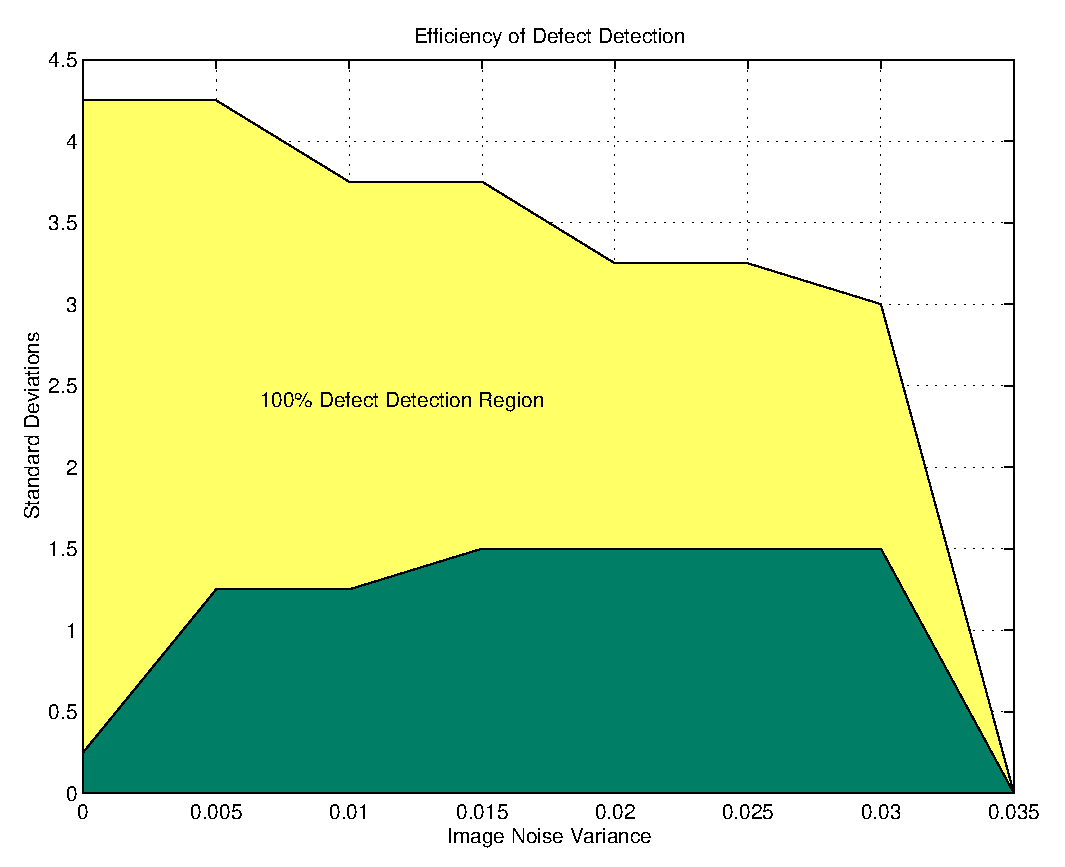
\includegraphics[width=\figwidth, totalheight=\figheight]{epsfig}}
    \hfill
    \subfigure[A subfigure.]{
    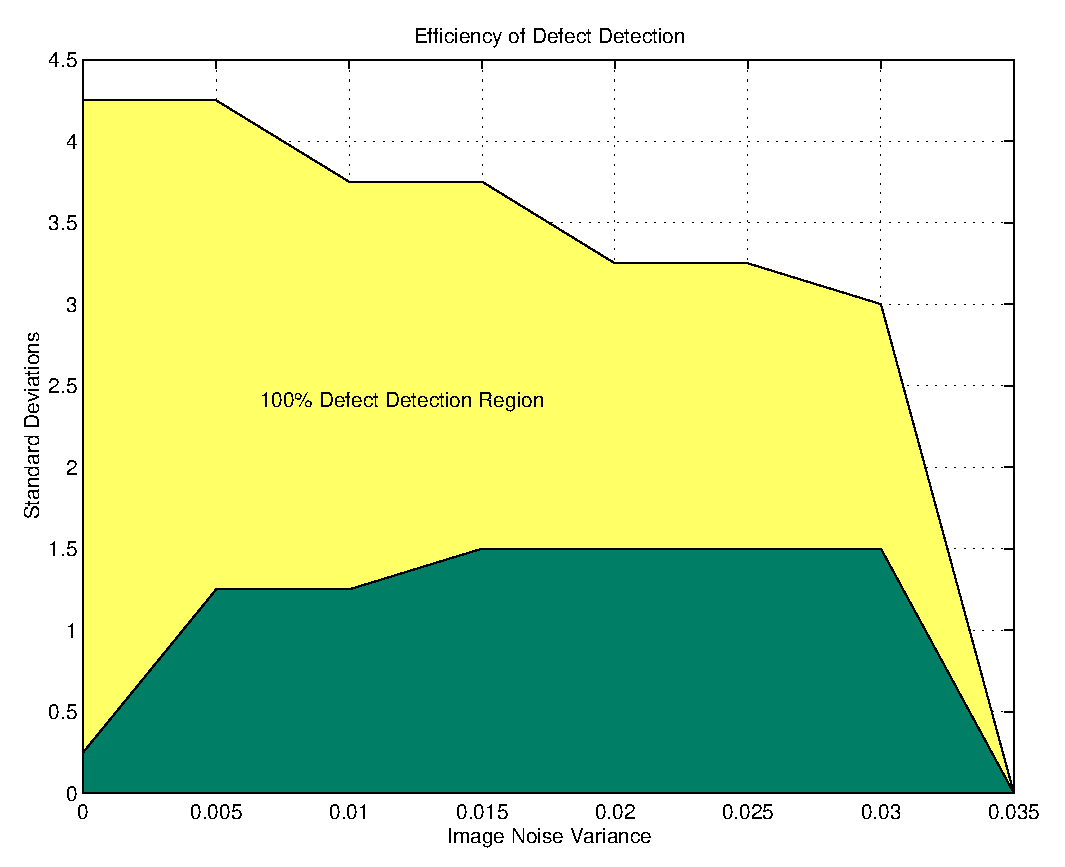
\includegraphics[width=\figwidth, totalheight=\figheight]{epsfig}} \\
    \subfigure[A subfigure.]{
    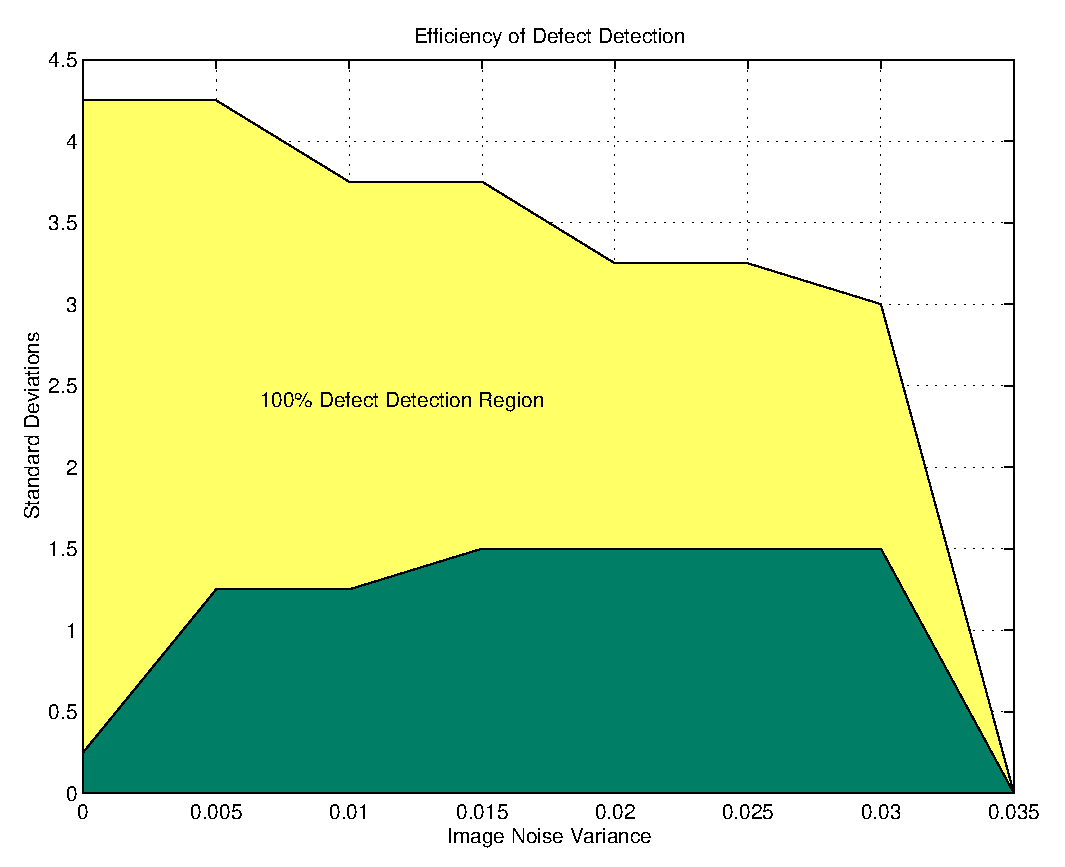
\includegraphics[width=\figwidth, totalheight=\figheight]{epsfig}}
    \hfill
    \subfigure[A subfigure.]{
    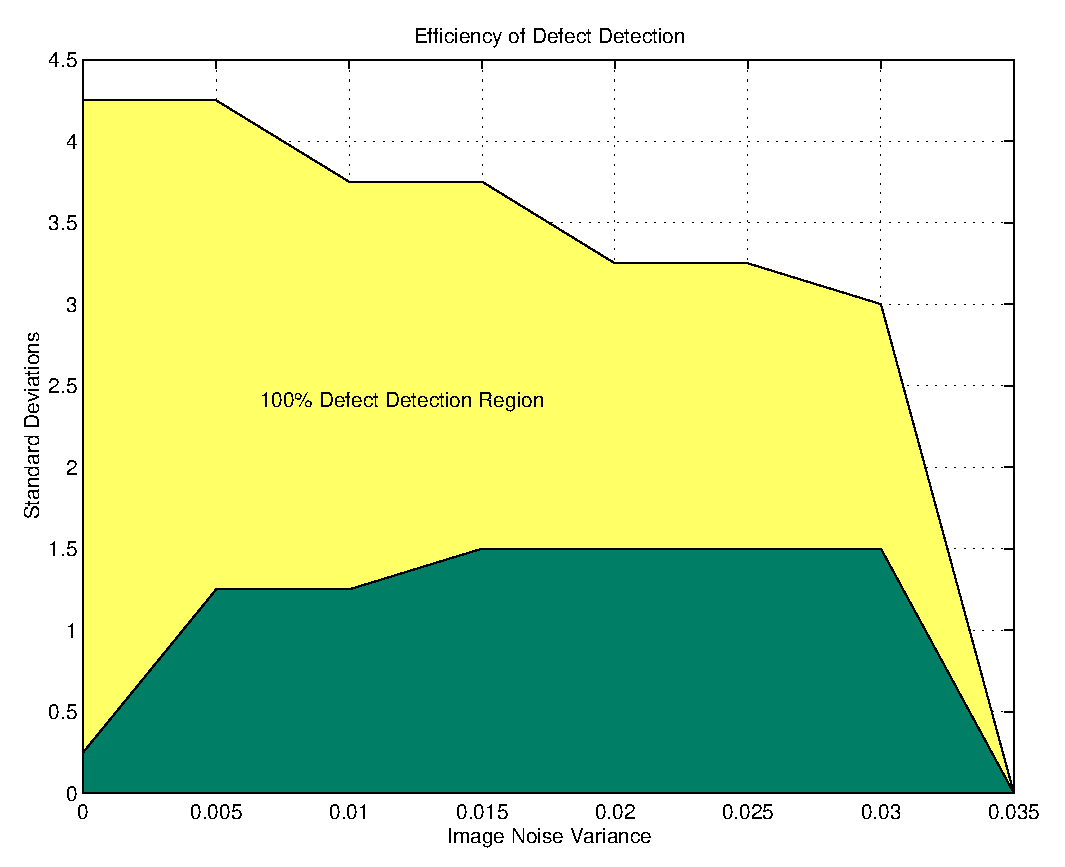
\includegraphics[width=\figwidth, totalheight=\figheight]{epsfig}}
    \hfill
    \subfigure[A subfigure.]{
    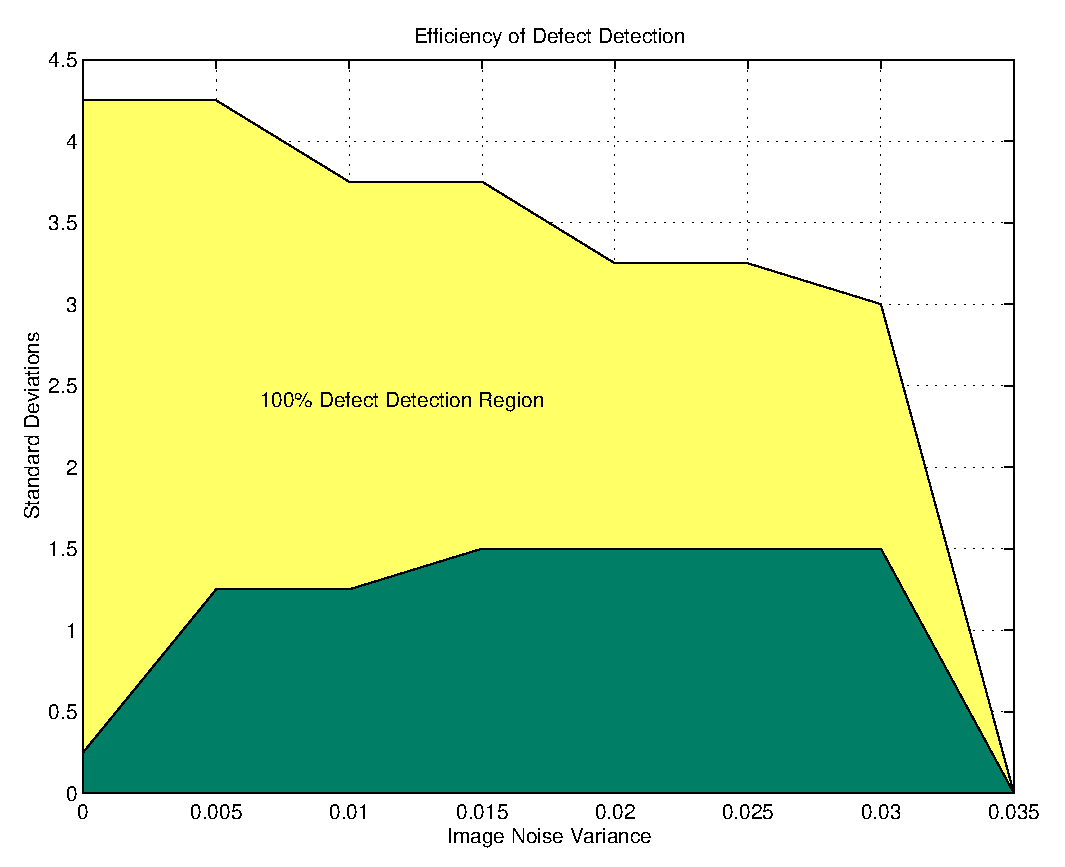
\includegraphics[width=\figwidth, totalheight=\figheight]{epsfig}} \\
    \subfigure[A subfigure.]{
    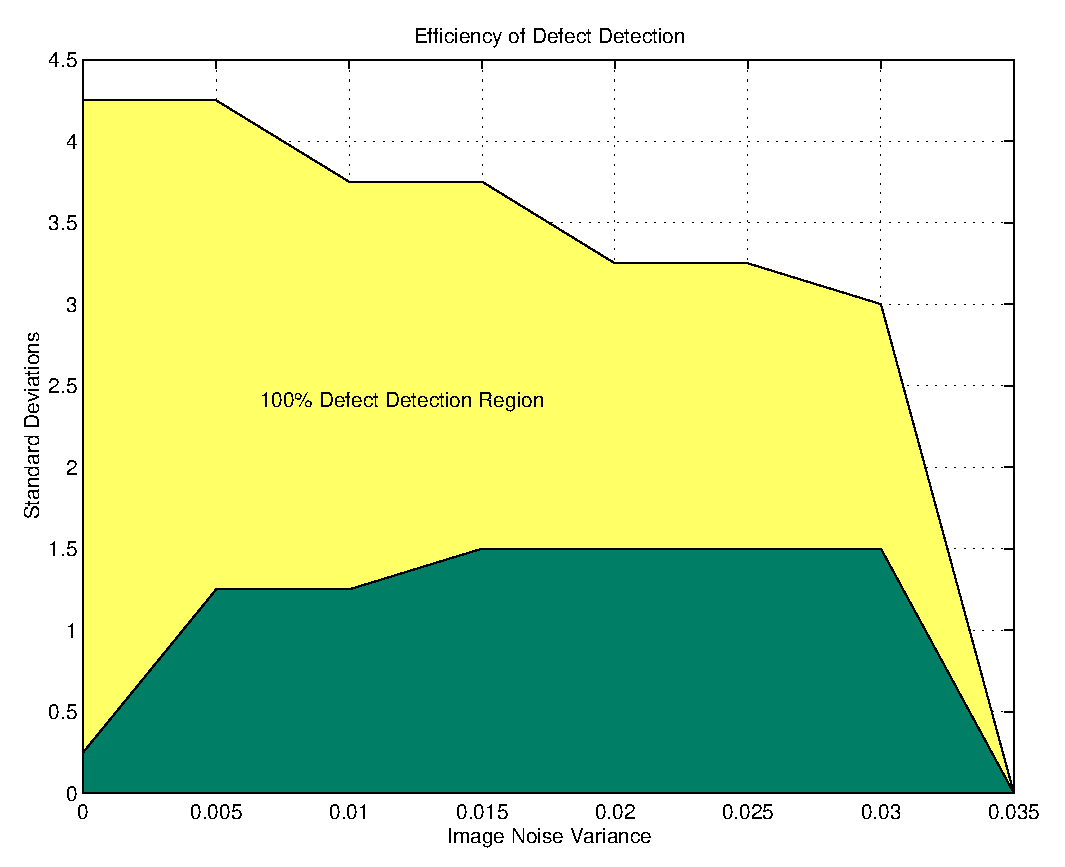
\includegraphics[width=\figwidth, totalheight=\figheight]{epsfig}}
    \hfill
    \subfigure[A subfigure.]{
    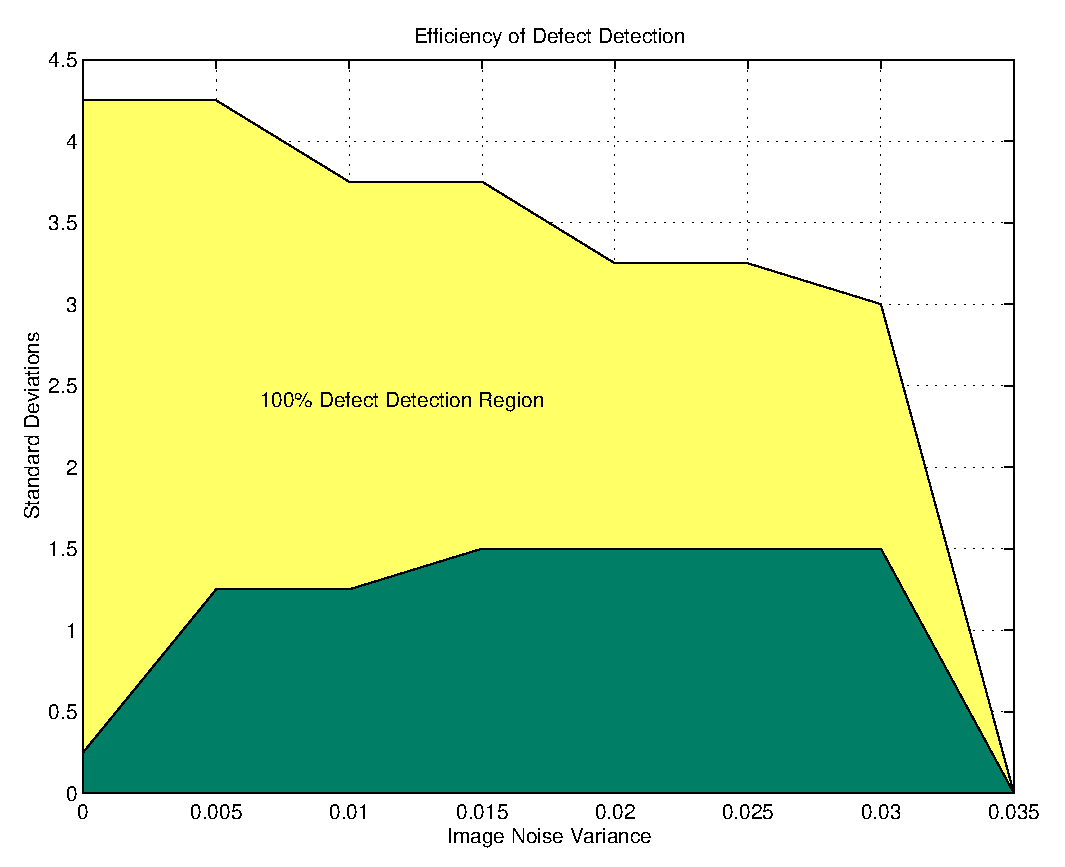
\includegraphics[width=\figwidth, totalheight=\figheight]{epsfig}}
    \hfill
    \subfigure[A subfigure.]{
    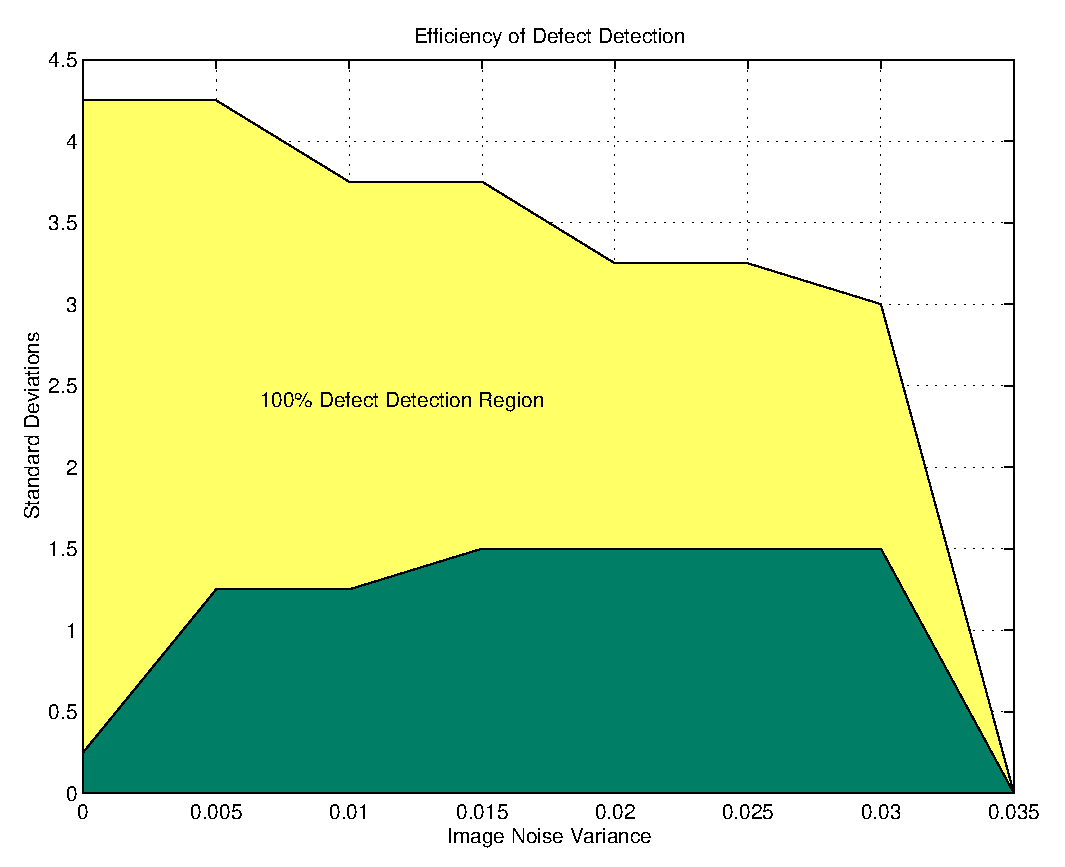
\includegraphics[angle=45, width=\figwidth,
    totalheight=\figheight]{epsfig}}

    \caption{This is where your caption text goes.
    Optional parameters causing the aspect ratio to be
    disregarded.}\label{fig:1b}
\end{figure}
\end{verbatim}


\begin{figure}
\SetFigLayout{3}{3}
    \subfigure[A subfigure.]{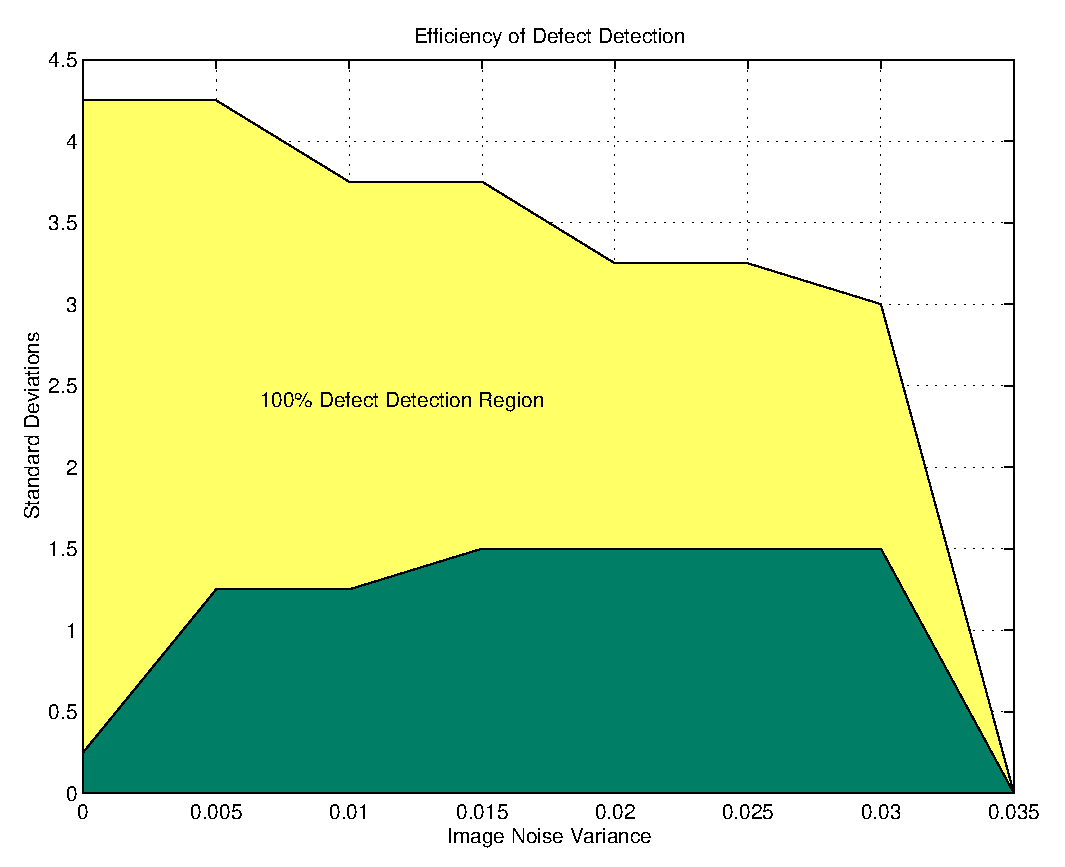
\includegraphics{epsfig}}
    \hfill
    \subfigure[A subfigure.]{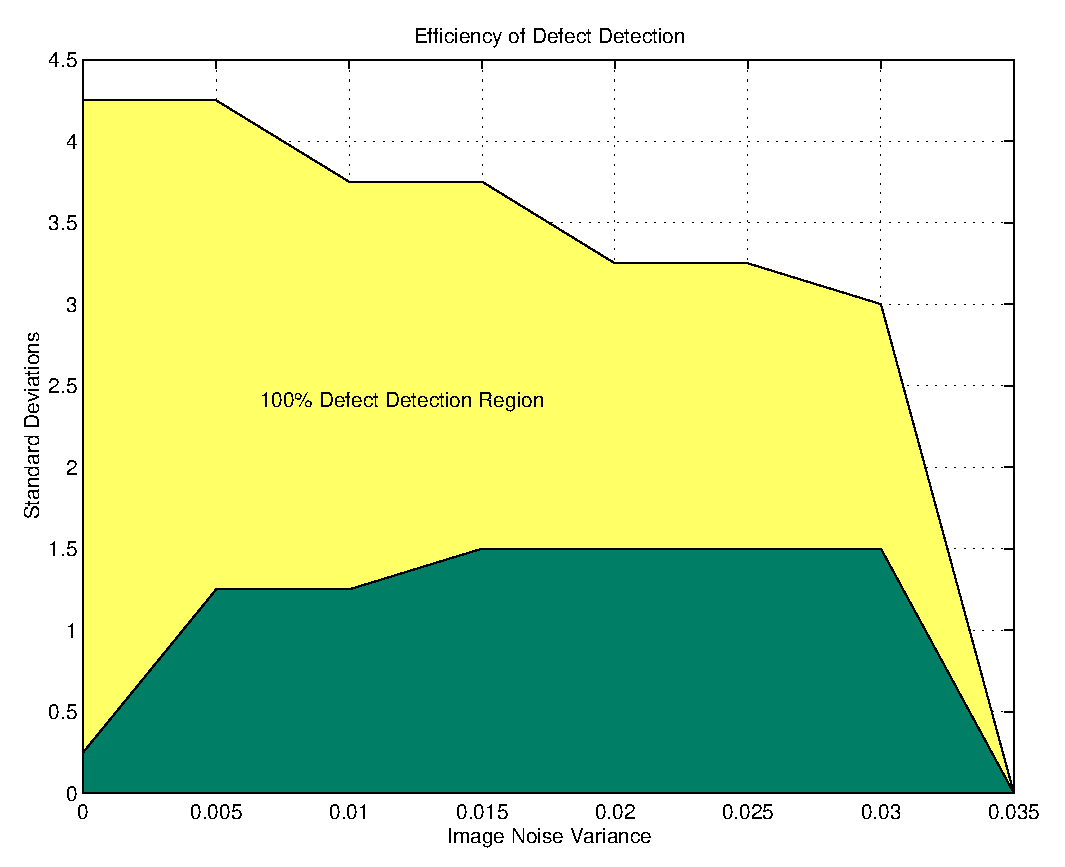
\includegraphics{epsfig}}
    \hfill
    \subfigure[A subfigure.]{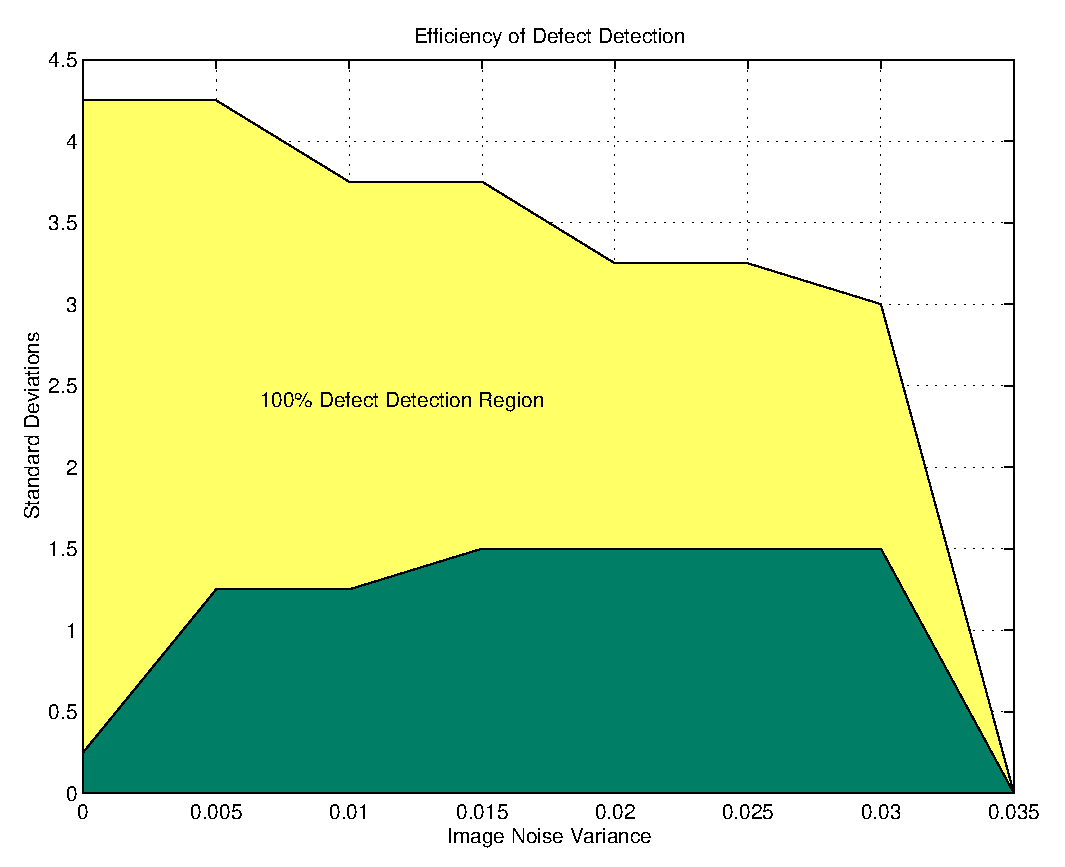
\includegraphics{epsfig}} \\
    \subfigure[A subfigure.]{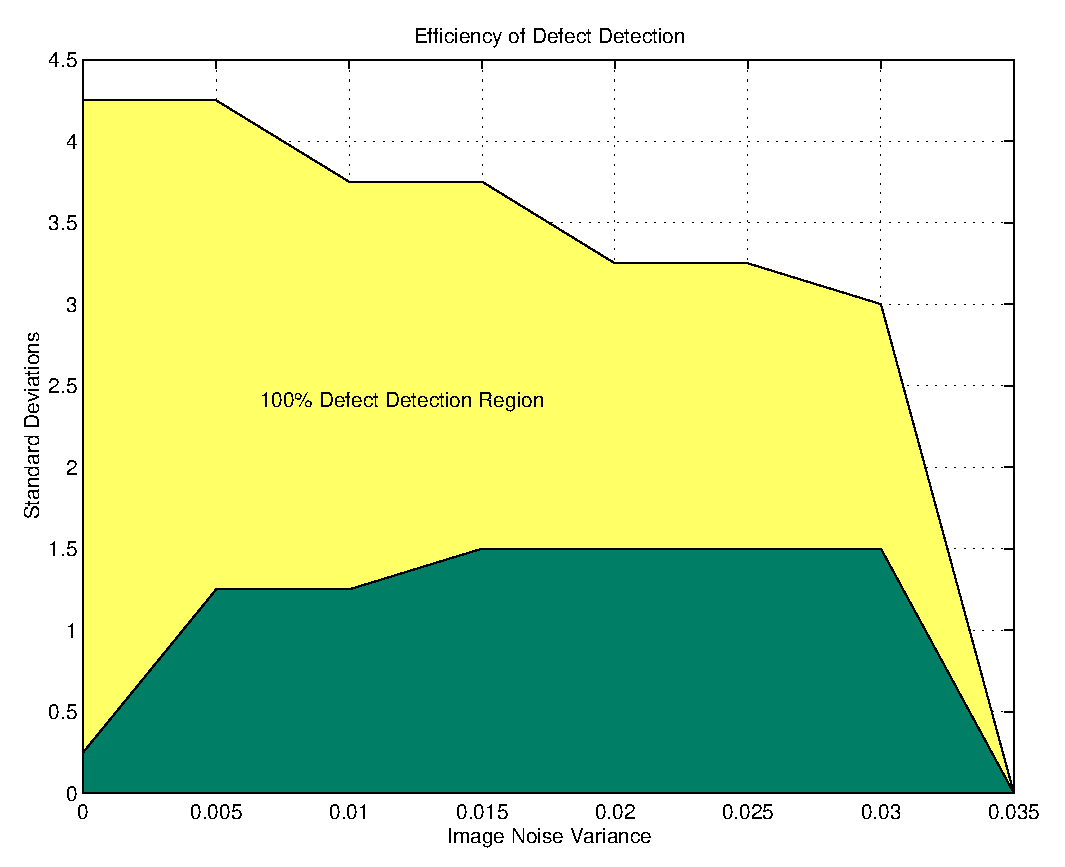
\includegraphics{epsfig}}
    \hfill
    \subfigure[A subfigure.]{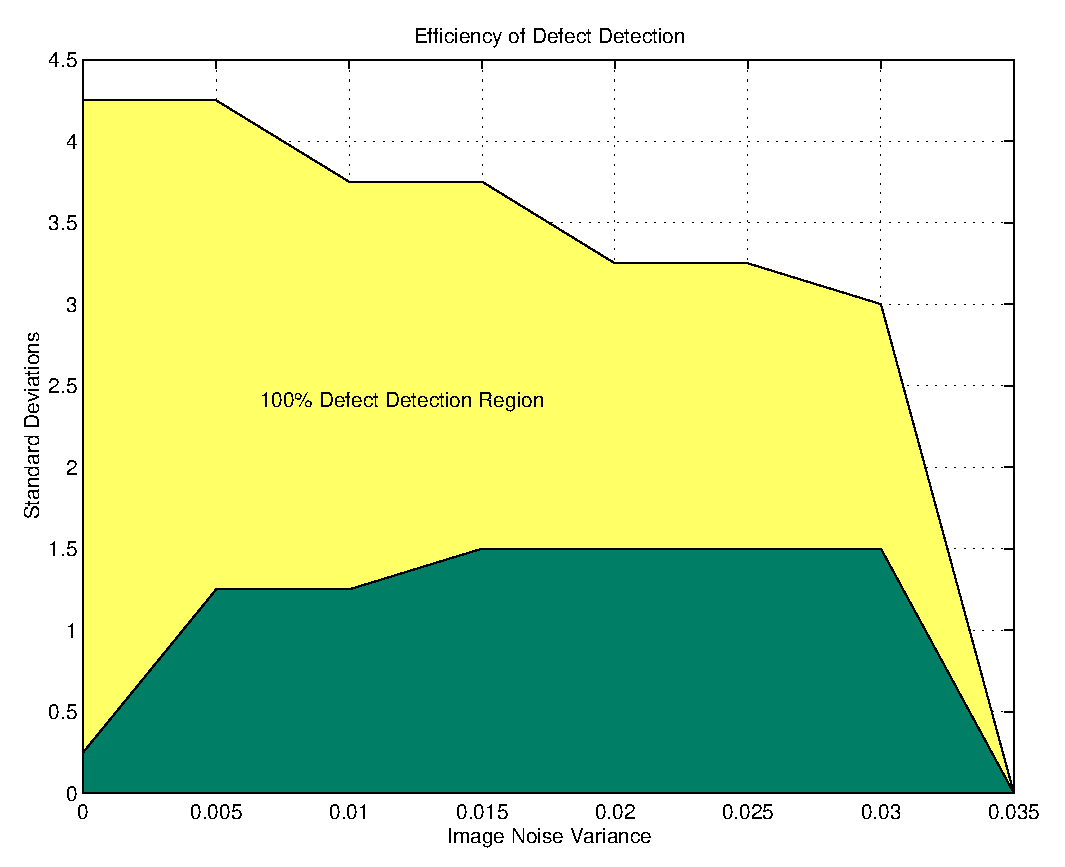
\includegraphics{epsfig}}
    \hfill
    \subfigure[A subfigure.]{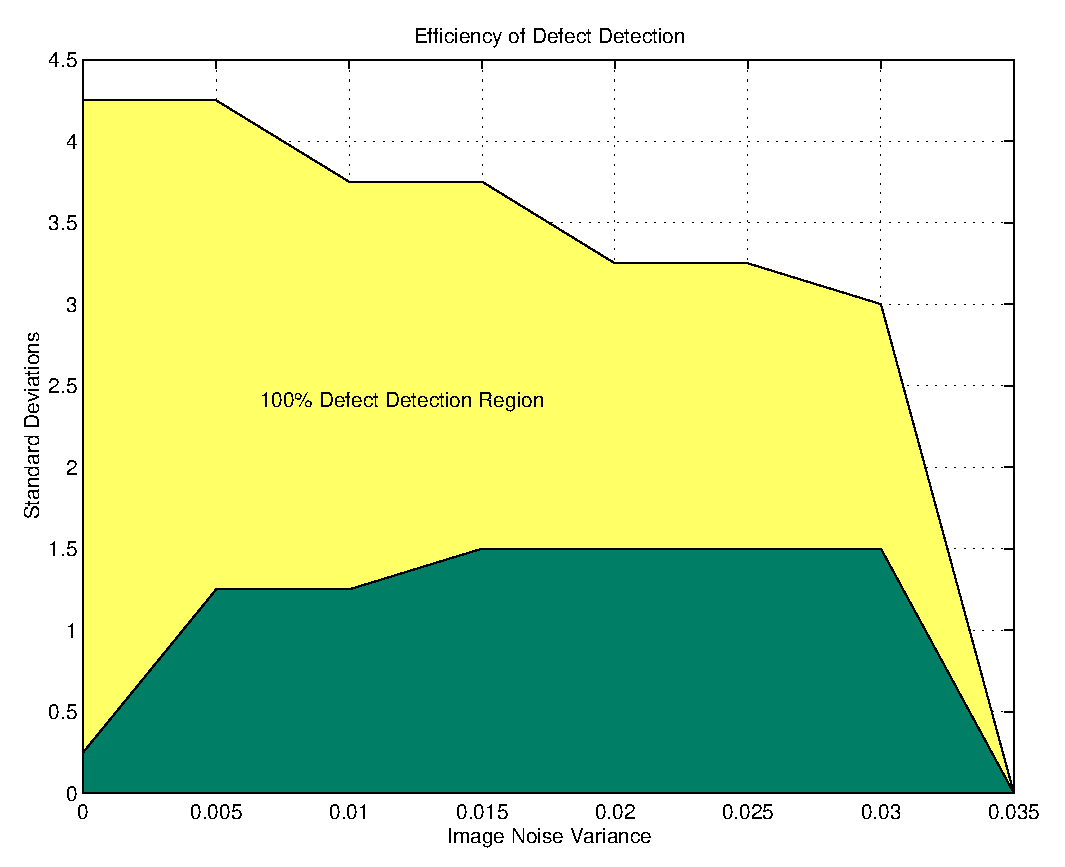
\includegraphics{epsfig}} \\
    \subfigure[A subfigure.]{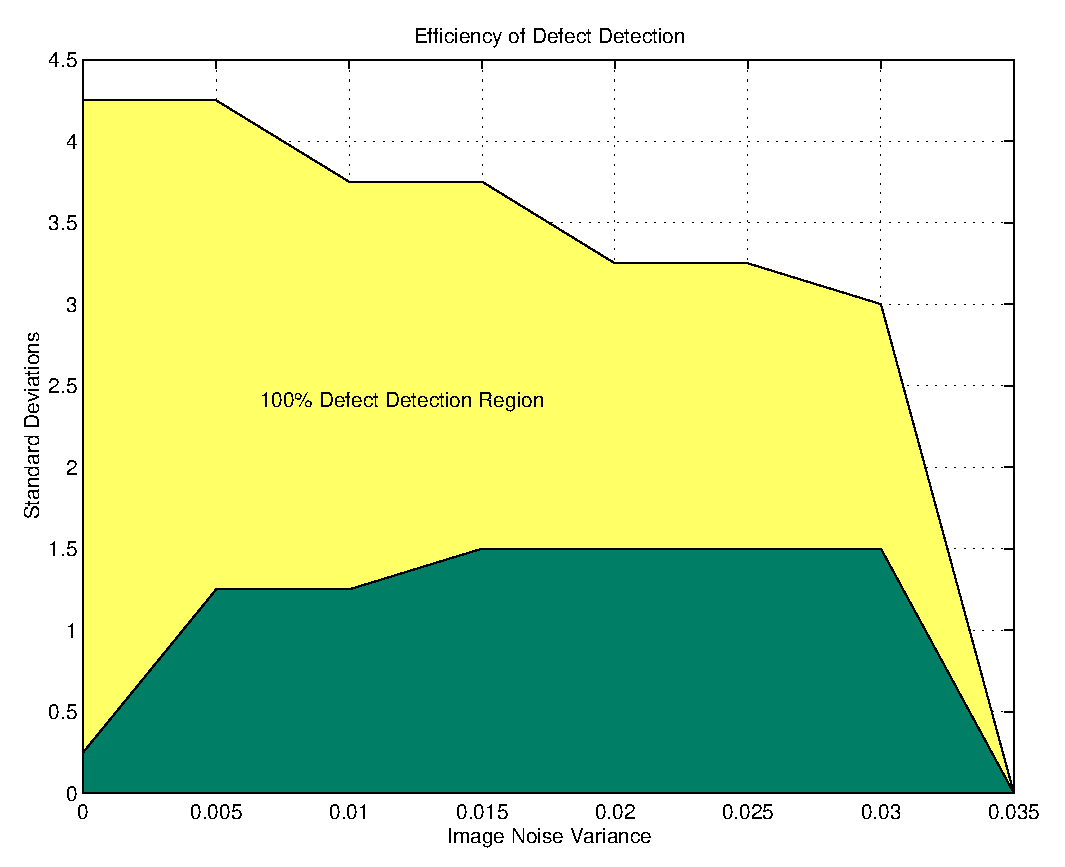
\includegraphics{epsfig}}
    \hfill
    \subfigure[A subfigure.]{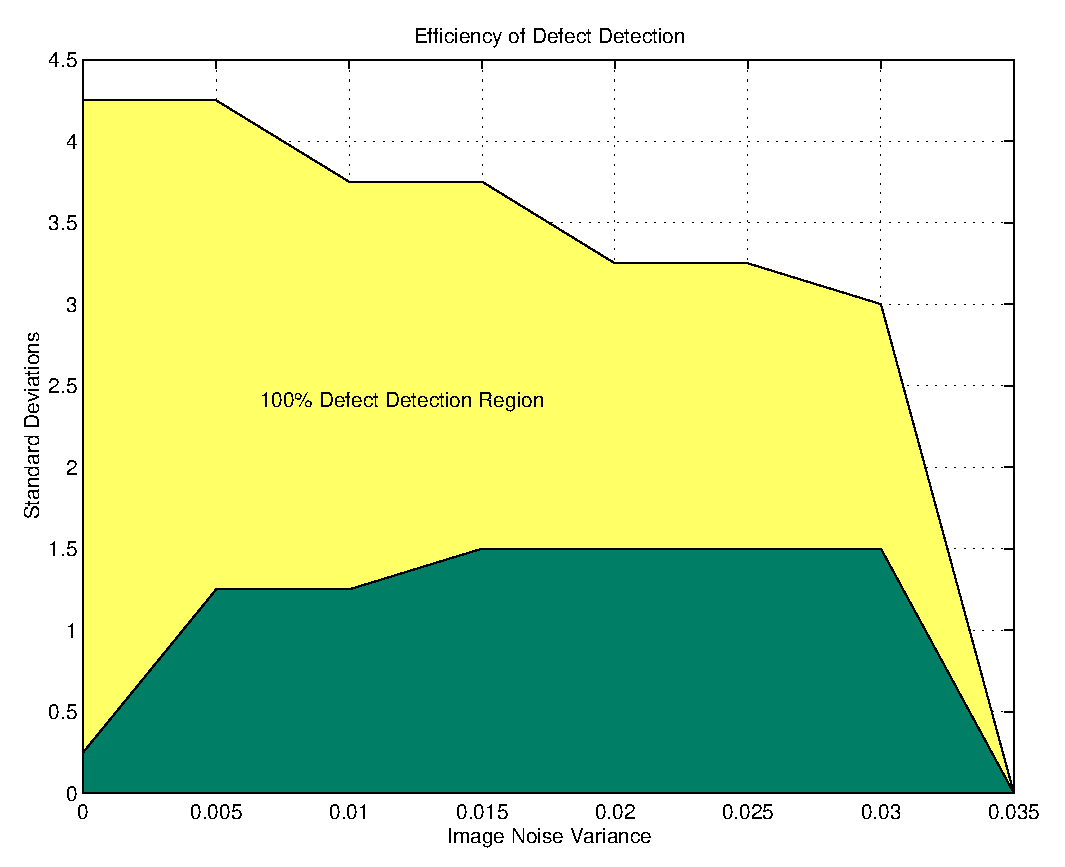
\includegraphics{epsfig}}
    \hfill
    \subfigure[A subfigure.]{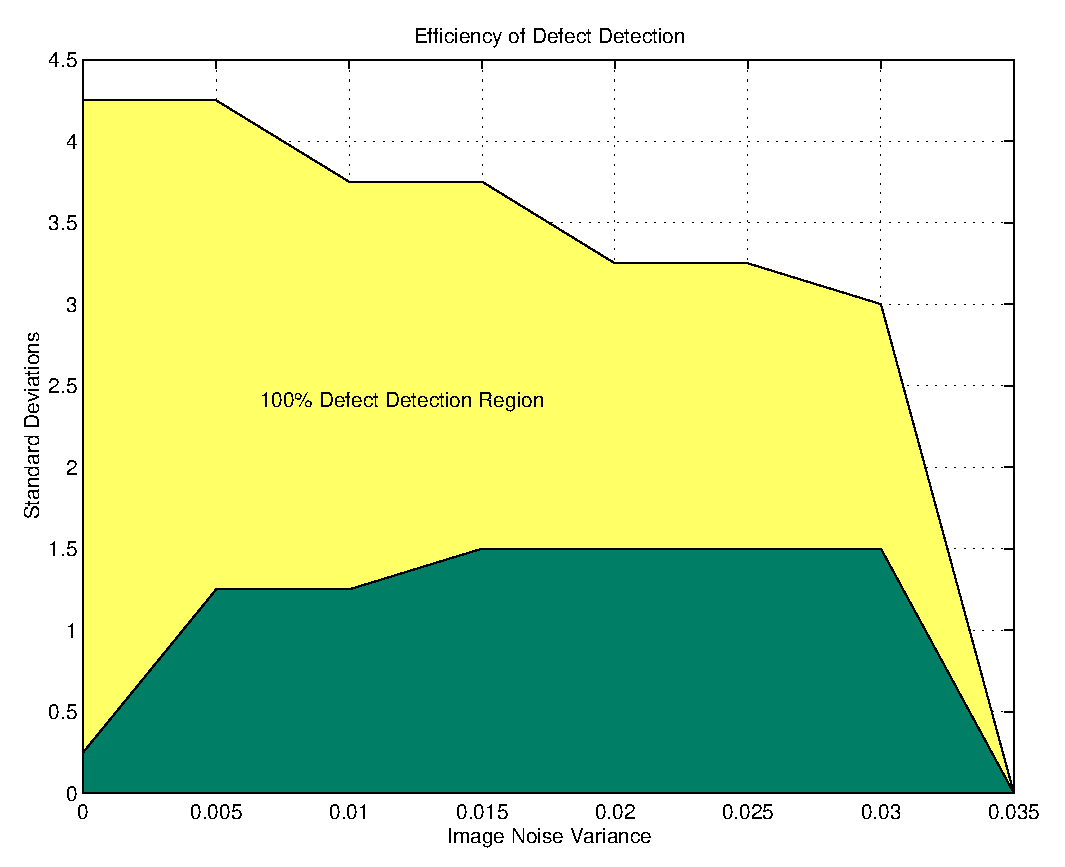
\includegraphics[angle=45, width=\figwidth, totalheight=\figheight, keepaspectratio]{epsfig}}
    \caption{This is where your caption text goes. No
    optional parameters.}\label{fig:1}
\end{figure}

\begin{figure}
\SetFigLayout{3}{3}
    \subfigure[A subfigure.]{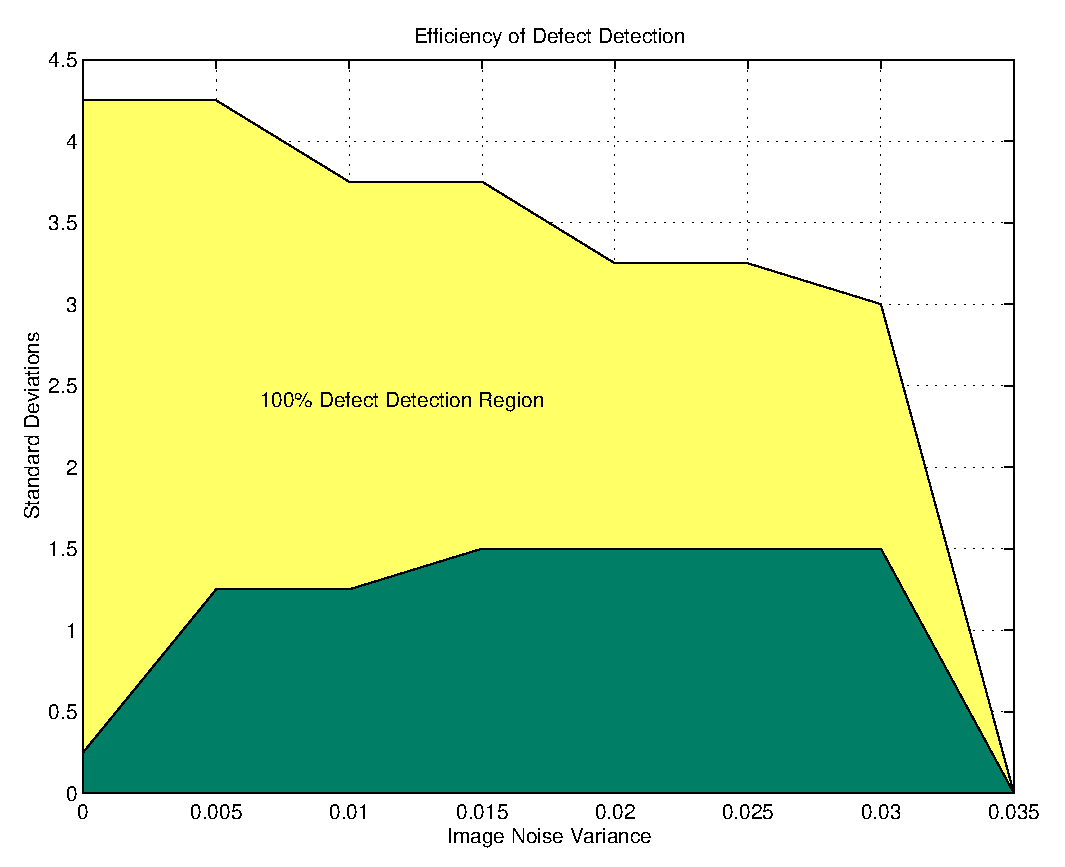
\includegraphics[width=\figwidth, totalheight=\figheight]{epsfig}}
    \hfill
    \subfigure[A subfigure.]{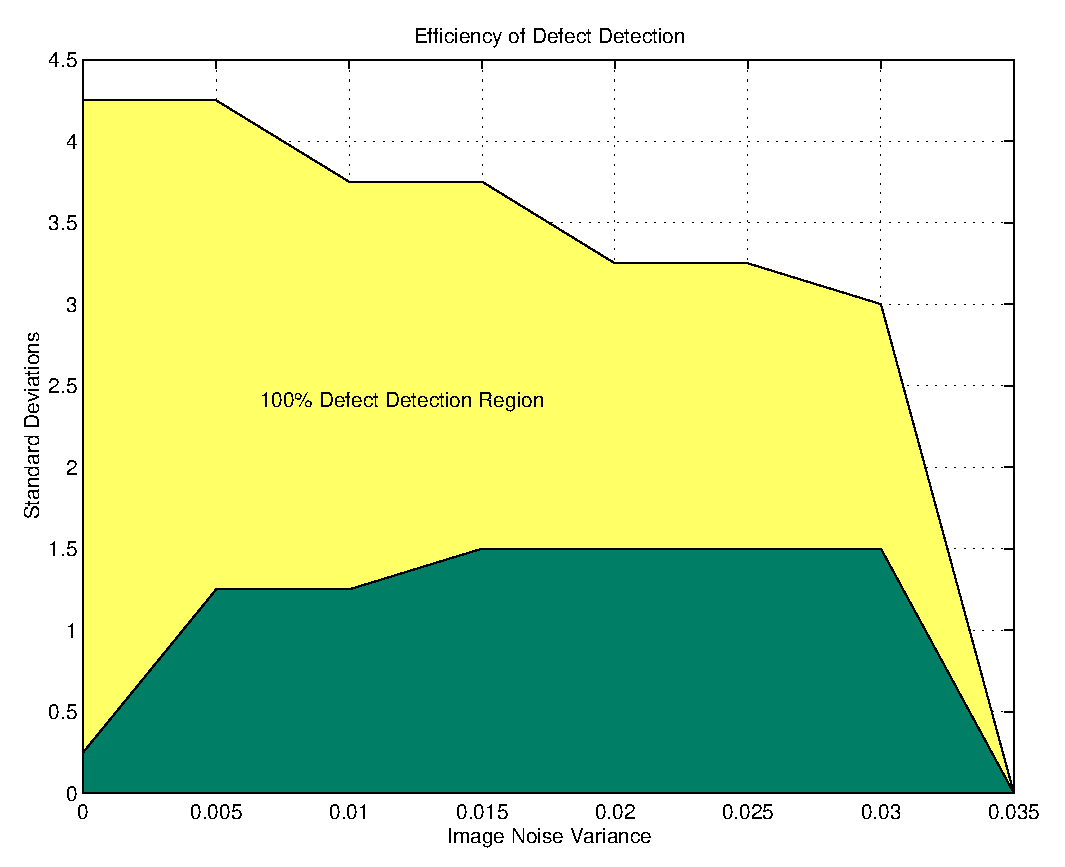
\includegraphics[width=\figwidth, totalheight=\figheight]{epsfig}}
    \hfill
    \subfigure[A subfigure.]{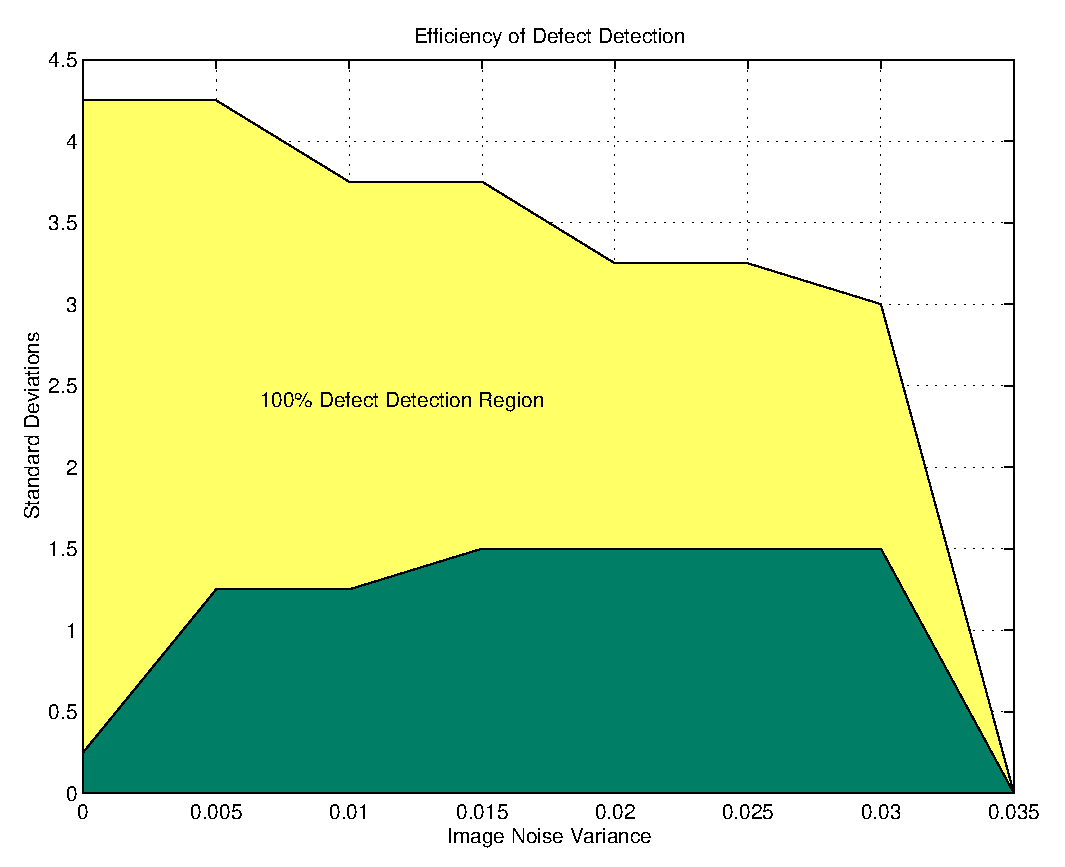
\includegraphics[width=\figwidth, totalheight=\figheight]{epsfig}} \\
    \subfigure[A subfigure.]{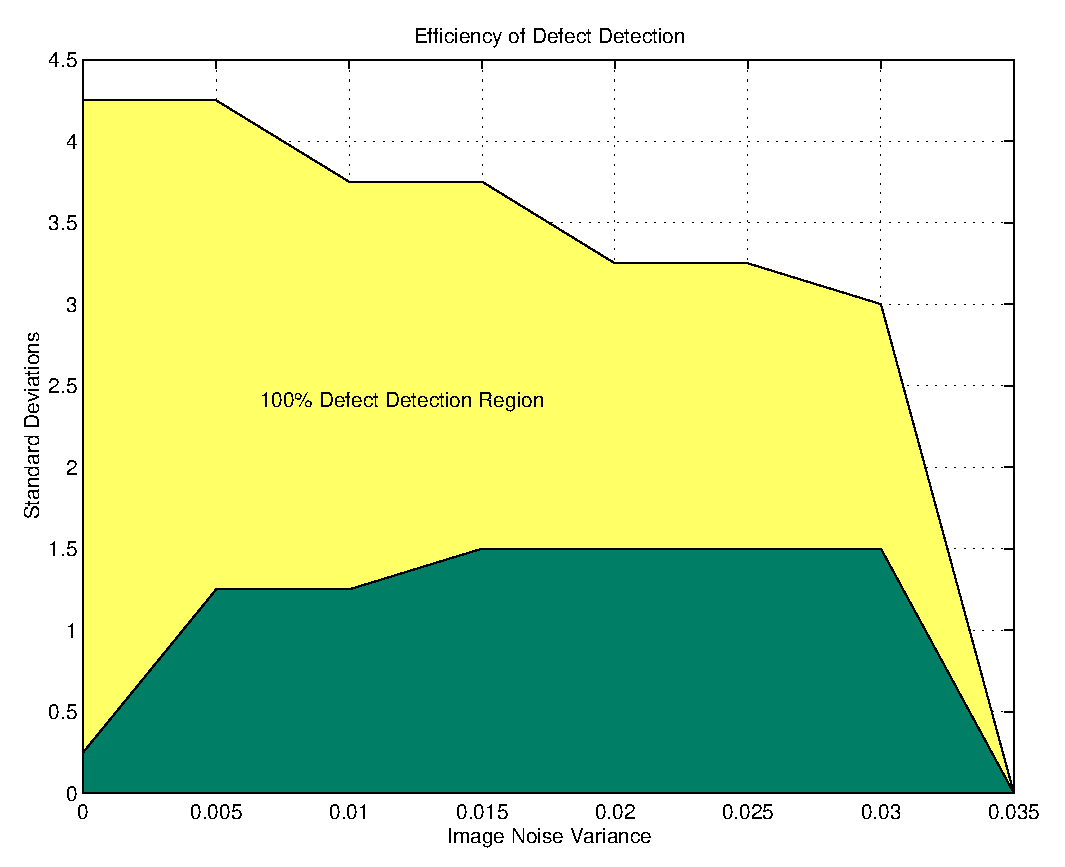
\includegraphics[width=\figwidth, totalheight=\figheight]{epsfig}}
    \hfill
    \subfigure[A subfigure.]{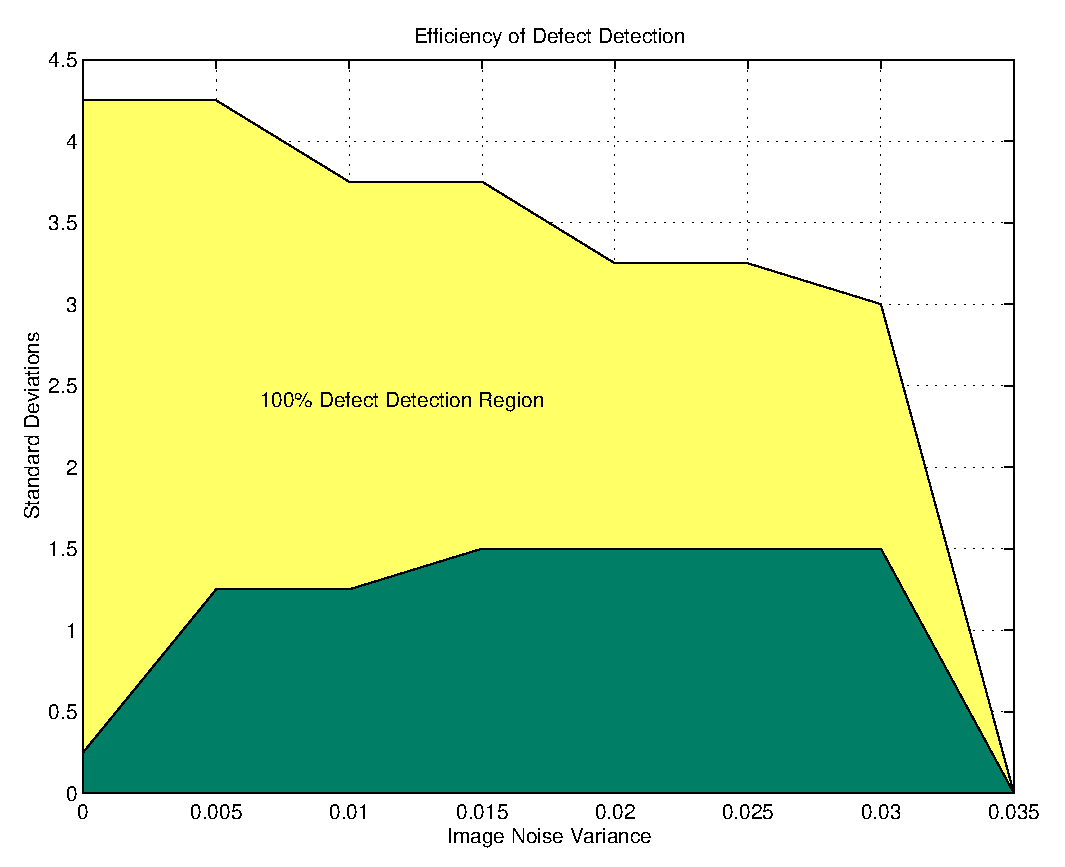
\includegraphics[width=\figwidth, totalheight=\figheight]{epsfig}}
    \hfill
    \subfigure[A subfigure.]{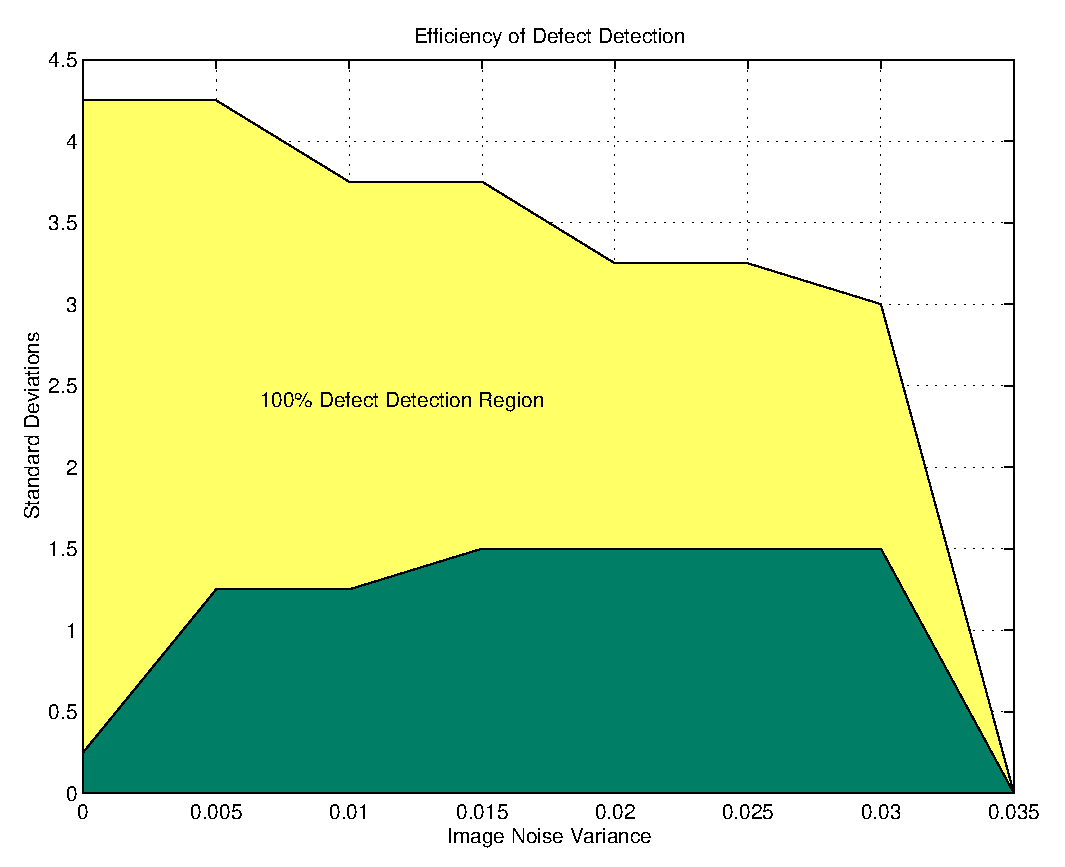
\includegraphics[width=\figwidth, totalheight=\figheight]{epsfig}} \\
    \subfigure[A subfigure.]{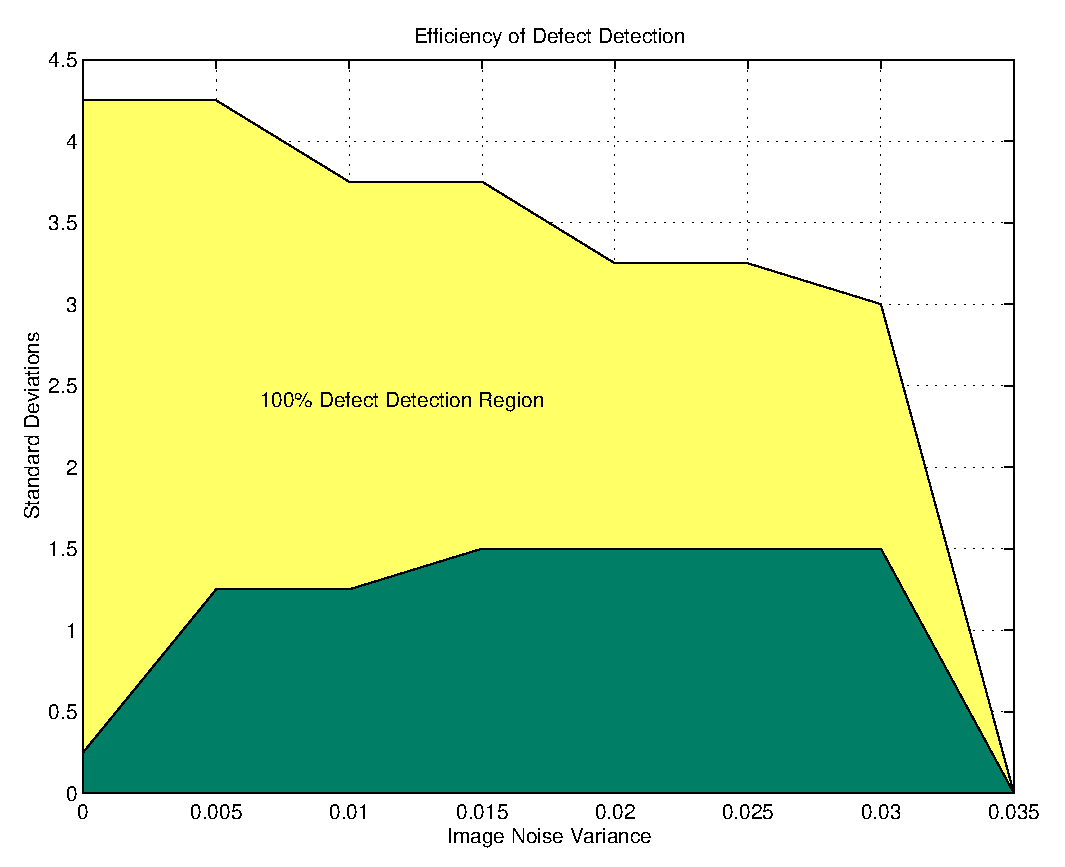
\includegraphics[width=\figwidth, totalheight=\figheight]{epsfig}}
    \hfill
    \subfigure[A subfigure.]{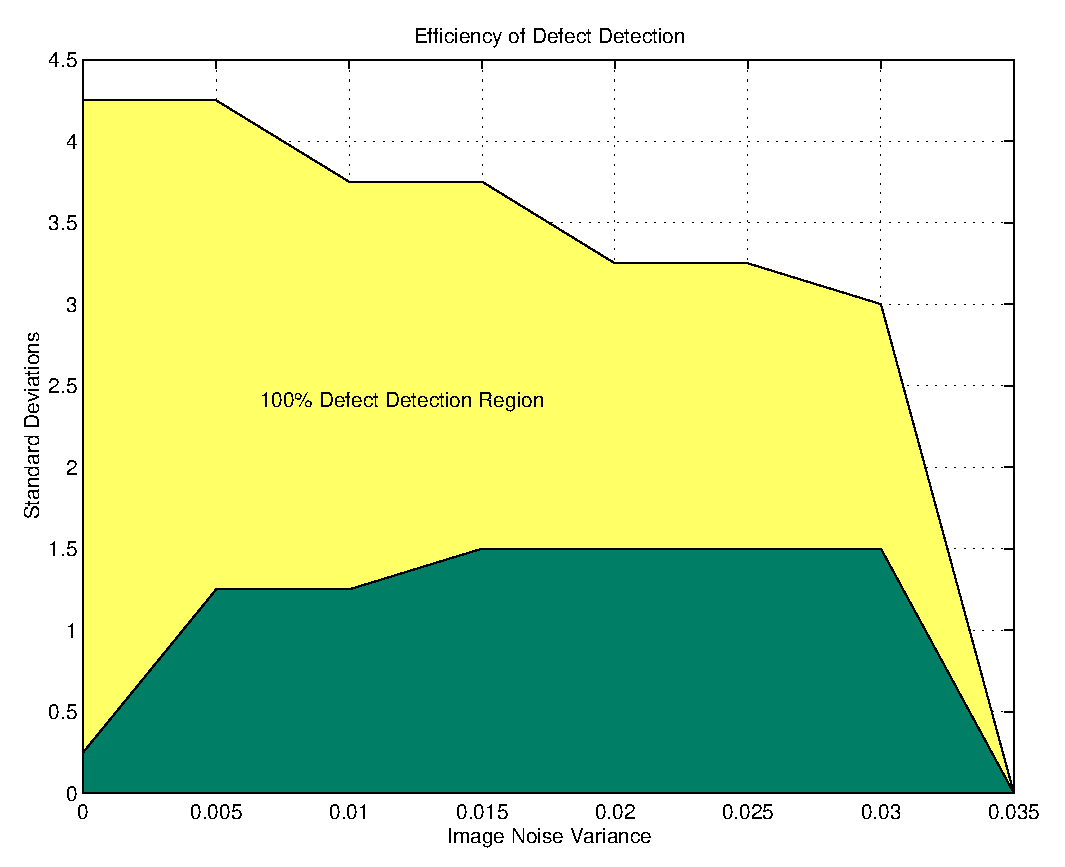
\includegraphics[width=\figwidth, totalheight=\figheight]{epsfig}}
    \hfill
    \subfigure[A subfigure.]{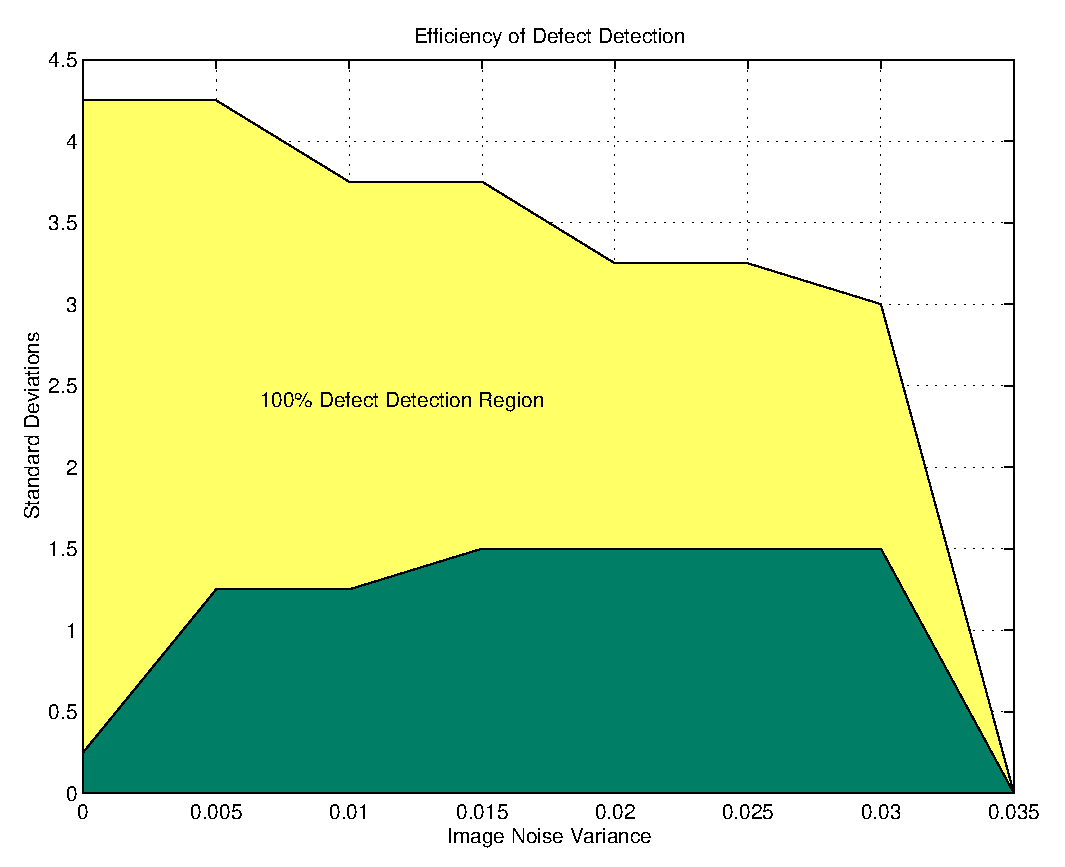
\includegraphics[angle=45, width=\figwidth, totalheight=\figheight]{epsfig}}
    \caption{This is where your caption text goes.
    Optional parameters causing the aspect ratio to be
    disregarded.}\label{fig:1b}
\end{figure}

The following code produces a graphic occupying the whole page
(maximally). The result is shown in Figures \ref{fig:2} and
\ref{fig:2b}.

\begin{verbatim}
\begin{figure}
    \SetFigLayout{1}{1}
    {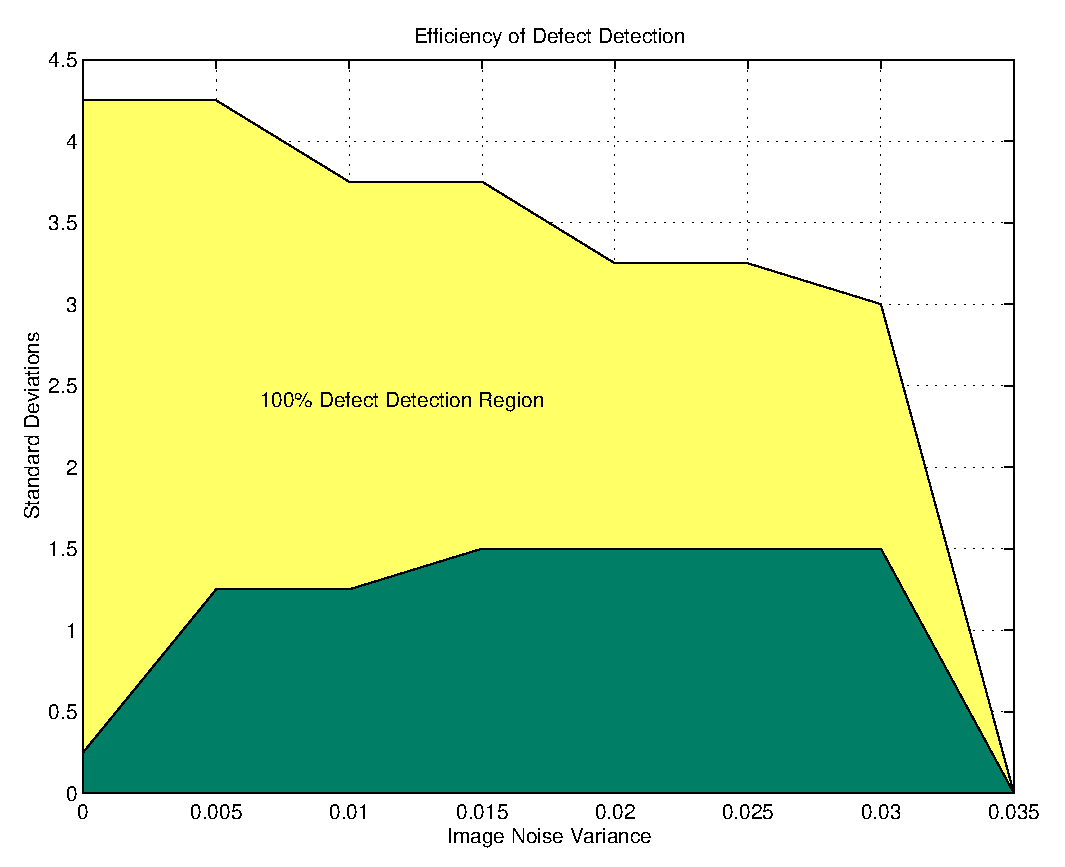
\includegraphics{epsfig}}
    \caption{A graphic meant to occupy a whole page.  Note
    that the aspect ratio is respected so the graphic
    can only occupy the whole text width.}
\end{figure}
\end{verbatim}

\begin{figure}
\SetFigLayout{1}{1} {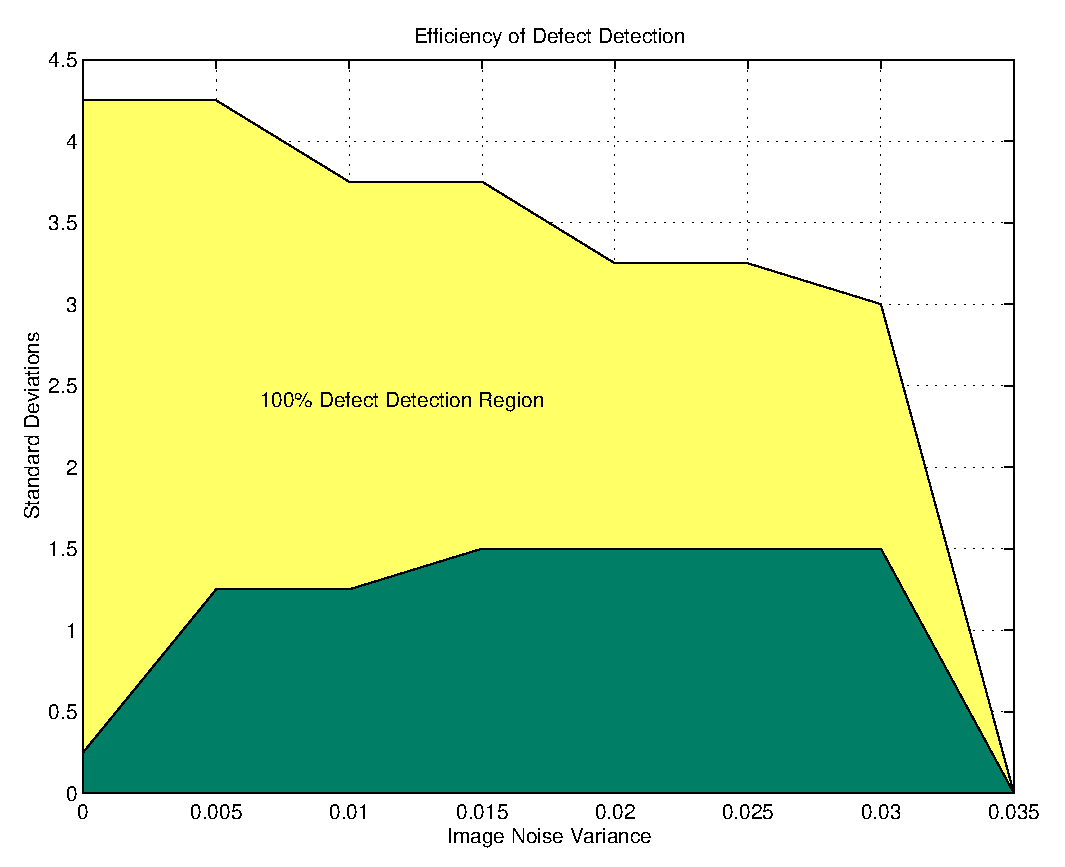
\includegraphics{epsfig}}
    \caption{A graphic meant to occupy a whole page.  Note
    that the aspect ratio is respected so the graphic
    can only
    occupy the whole text width.}\label{fig:2}
\end{figure}

\begin{verbatim}
\begin{figure}
    \SetFigLayout{1}{1}
    {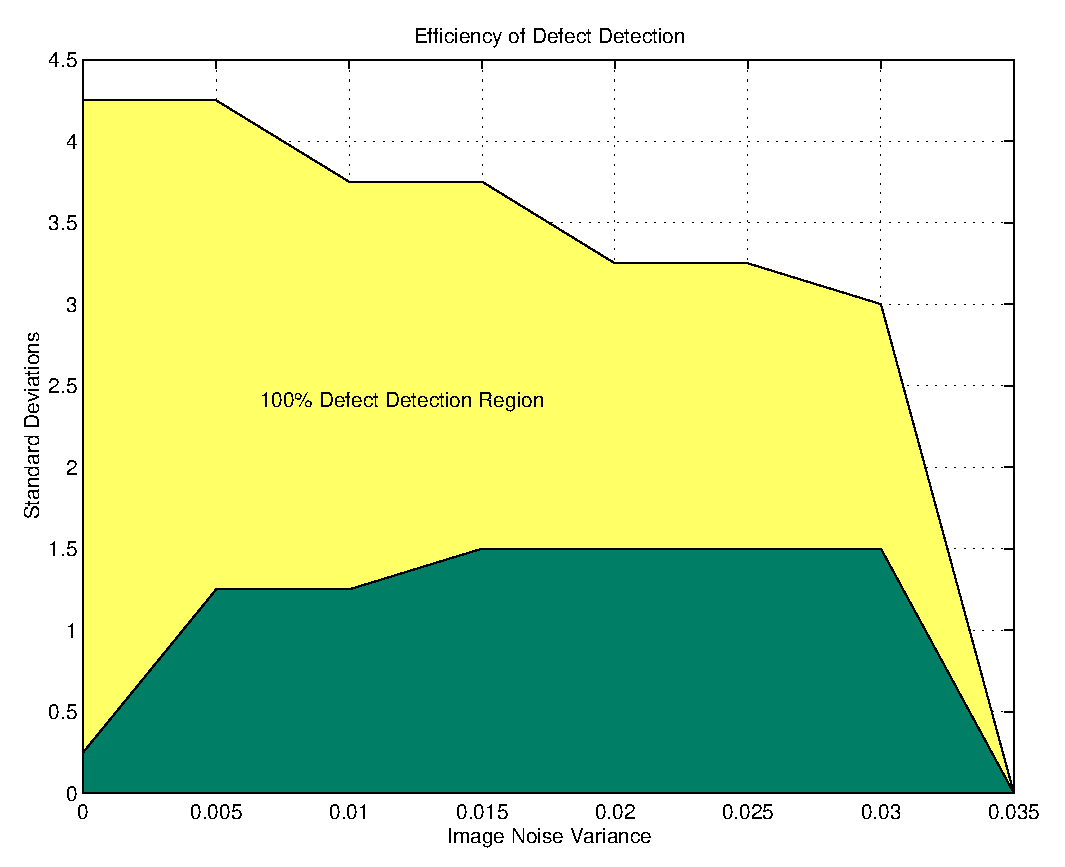
\includegraphics[%
    width=\figwidth, totalheight=\figheight]{epsfig}}
    \caption{Now the graphic occupies the whole page because
    we manually specified the parameters to the
    include graphics command which omitted keepaspectratio.}
\end{figure}
\end{verbatim}

\begin{figure}
\SetFigLayout{1}{1} {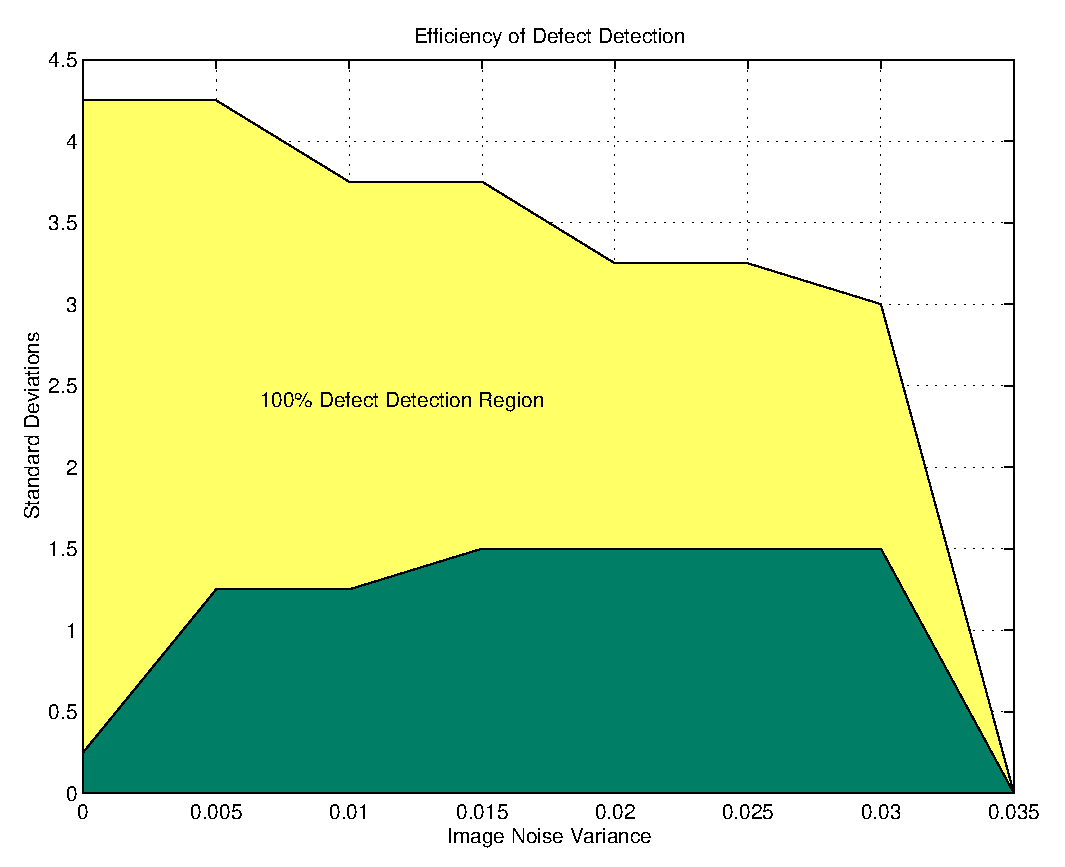
\includegraphics[width=\figwidth,
totalheight=\figheight]{epsfig}}
    \caption{Now the graphic occupies the whole page because
     we manually specified the parameters to the
    include graphics command which omitted keepaspectratio.}\label{fig:2b}
\end{figure}


The next figure is sized such that only two graphics occupy at
most half of the page, allowing for document text to flow onto the
rest of the page. The result is shown in Figure \ref{fig:3}.

\begin{verbatim}
\begin{figure}
    \centering
    \SetFigLayout[3]{2}{2}
    \subfigure[]{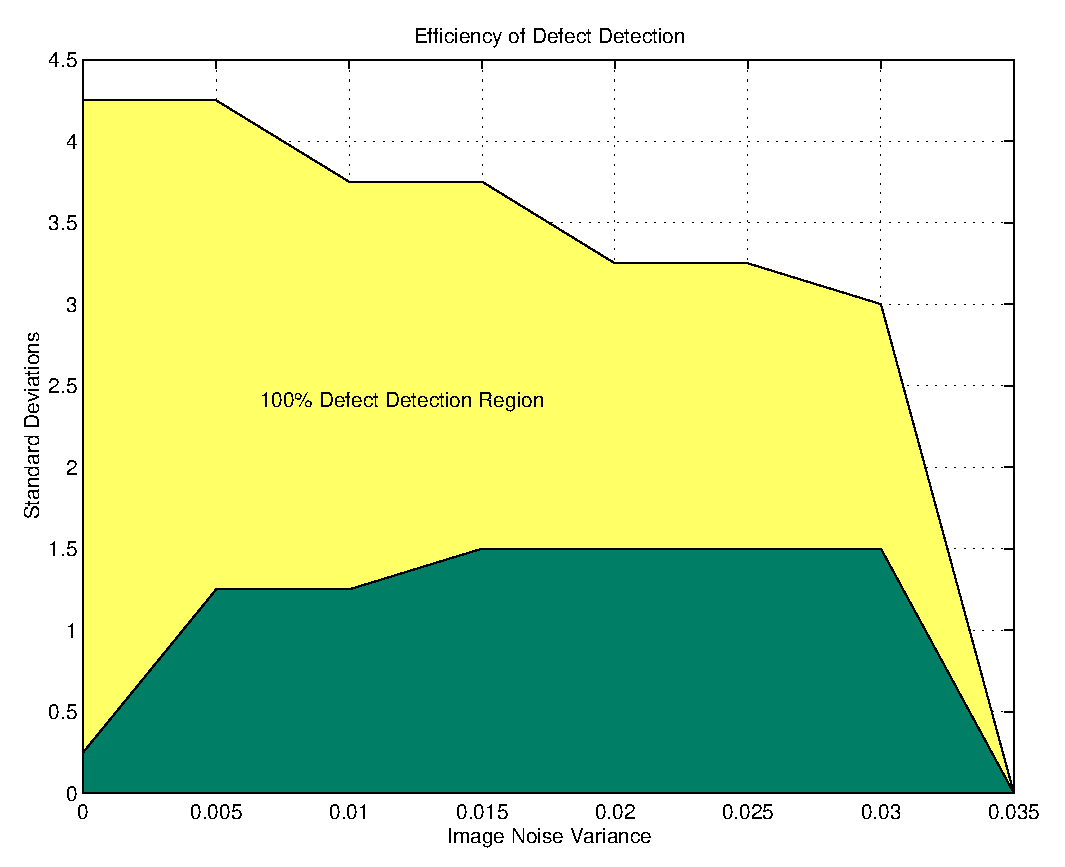
\includegraphics{epsfig}} \hfill
    \subfigure[]{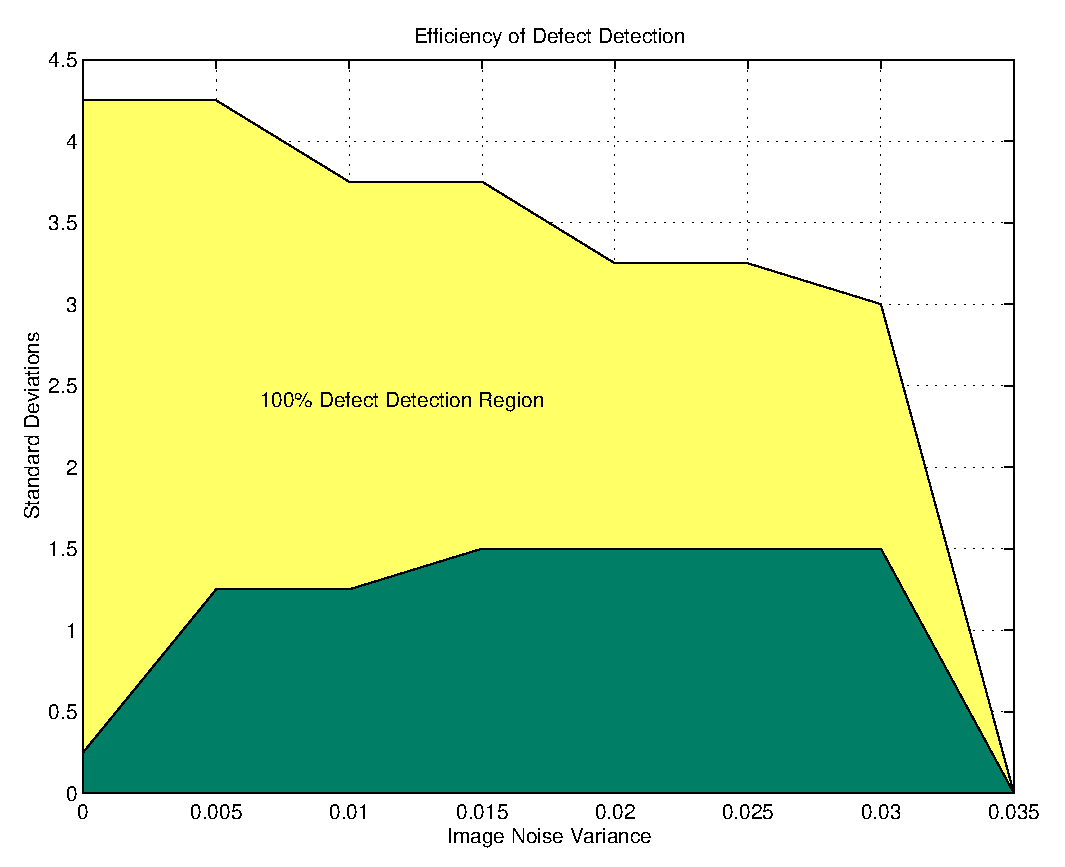
\includegraphics{epsfig}}
\end{figure}
\end{verbatim}
\
\begin{figure}
    \centering
    \SetFigLayout[3]{2}{2}
    \subfigure[]{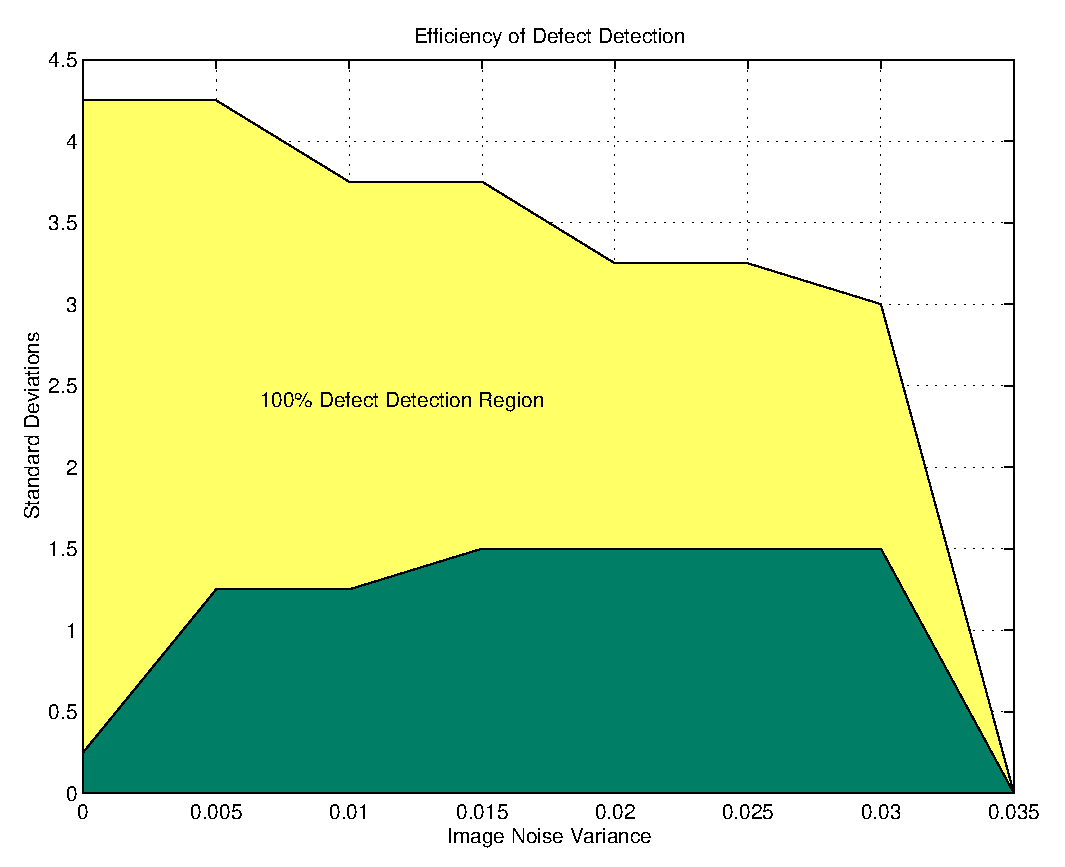
\includegraphics{epsfig}} \hfill
    \subfigure[]{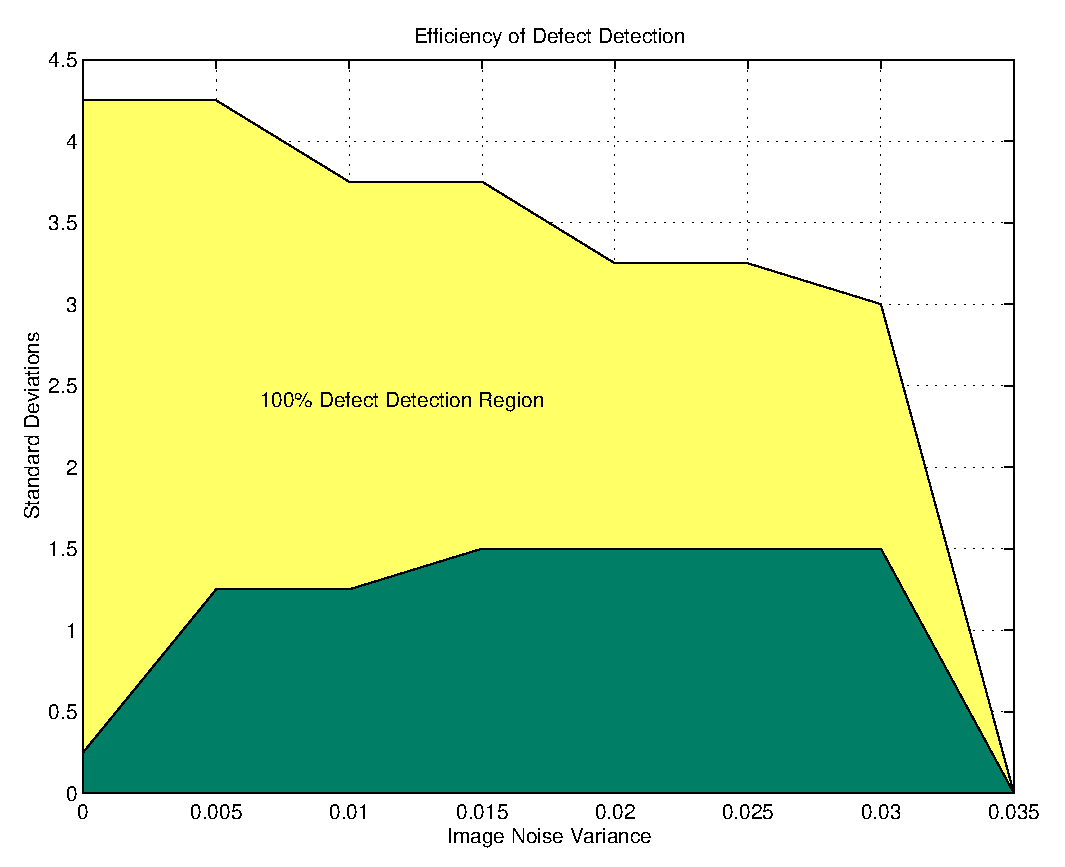
\includegraphics{epsfig}}
    \caption{This is where your caption text goes.}\label{fig:3}
\end{figure}



The following code is an example of including a full size graphic
with a long caption.  The option 5 tells the algorithm to leave
space for 5 extra lines of caption text.  Without providing
telling the algorithm that the caption is expected to take at most
5 extra lines than the one allowed an over full box would occur on
the page.
\begin{verbatim}

\begin{figure}
    \SetFigLayout[5]{1}{1}
    {\includegraphics[%
    width=\figwidth, totalheight=\figheight]{epsfig}}
    \caption{This is where your caption text goes.
    This is where your caption text goes.
    This is where your caption text goes.
    This is where your caption text goes.
    This is where your caption text goes.
    This is where your caption text goes.
    This is where your caption text goes.}
\end{figure}
\end{verbatim}

\begin{figure}
\SetFigLayout[5]{1}{1} {\includegraphics[%
    width=\figwidth, totalheight=\figheight]{epsfig}}
    \caption{This is where your caption text goes.
    This is where your caption text goes.
    This is where your caption text goes.
    This is where your caption text goes.
    This is where your caption text goes.
    This is where your caption text goes.
    This is where your caption text goes.}\label{fig:4}
\end{figure}

Figure \ref{fig:5} shows how you can mix and match the sizes
relative graphic sizes.

\begin{verbatim}
\begin{figure}
    \centering
    \SetFigLayout[3]{2}{2}
    \subfigure[]{\includegraphics{epsfig}} \hfill
    \subfigure[]{\includegraphics{epsfig}}
    %Now change the size mid way
    \SetFigLayout[3]{2}{1}
    \subfigure[]{\includegraphics{epsfig}}
    \caption{This is where your caption text goes.}
\end{figure}
\end{verbatim}

\begin{figure}
    \centering
    \SetFigLayout[3]{2}{2}
    \subfigure[]{\includegraphics{epsfig}} \hfill
    \subfigure[]{\includegraphics{epsfig}}
    \SetFigLayout[3]{2}{1}
    \subfigure[]{\includegraphics{epsfig}}
    \caption{This is where your caption text goes.}\label{fig:5}
\end{figure}

Finally, we can utilize the \verb"\figwidth" and \verb"\figheight"
commands for other environments like tables as shown in Table
\ref{tab:1}.  The code that produced the tables was,

\begin{verbatim}
\begin{table}
    \caption{Two tables that are half page width}\label{tab:1}
    \SetFigLayout{1}{2}
\begin{tabular*}{\figwidth}{ccc}
\hline
  A & B & C \\ \hline
  555 & 111 & 333 \\
  555 & 111 & 333 \\
  555 & 111 & 333 \\
  555 & 111 & 333 \\
  555 & 111 & 333 \\
      \hline
 \end{tabular*}
    \hfill
\begin{tabular*}{\figwidth}{ccc}
\hline
  A & B & C \\ \hline
  555 & 111 & 333 \\
  555 & 111 & 333 \\
  555 & 111 & 333 \\
  555 & 111 & 333 \\
  555 & 111 & 333 \\
      \hline
 \end{tabular*}

\end{table}
\end{verbatim}



\begin{table}
    \caption{Two tables that are half page width}\label{tab:1}
    \SetFigLayout{1}{2}
\begin{tabular*}{\figwidth}{ccc}
\hline
  A & B & C \\ \hline
  555 & 111 & 333 \\
  555 & 111 & 333 \\
  555 & 111 & 333 \\
  555 & 111 & 333 \\
  555 & 111 & 333 \\
      \hline
 \end{tabular*}
    \hfill
\begin{tabular*}{\figwidth}{ccc}
\hline
  A & B & C \\ \hline
  555 & 111 & 333 \\
  555 & 111 & 333 \\
  555 & 111 & 333 \\
  555 & 111 & 333 \\
  555 & 111 & 333 \\
      \hline
 \end{tabular*}

\end{table}



\section{Closing}
If you like this package, find bugs, or just have useful comments
please let the me know at atanbakuchi@hotmail.com.  Please note
that I am not a \TeX hack, just someone who had a wish for this
type of package and managed to find a solution.
\end{document}
